\documentclass[letterpaper, 10 pt, conference]{article} 
\usepackage[english]{babel}
\usepackage{amsmath,amssymb,amscd,amsthm} % variety of useful math macros
\usepackage[inner=1.5 cm, outer = 1.5 cm, top=1 cm, bottom = 1.5 cm]{geometry}
\usepackage{subcaption}
%For inserting graphics
\usepackage{graphicx}
\usepackage[dvipsnames]{xcolor}
\usepackage{listings}
\usepackage[utf8]{inputenc}
\usepackage{hyperref}
\usepackage{array, multirow}
\usepackage{lipsum}
%For diagrams
%\usepackage{tikz} 


\newcommand\N{\ensuremath{\mathcal{N}}}		%N for networks
\renewcommand{\P}{\ensuremath{\mathbb{P}}} %P for probability measures
\renewcommand{\iff}{\ensuremath{\Leftrightarrow}} %Shorter \iff 

%\newtheorem{theorem}{Theorem}
\newtheorem{prop}{Proposition}
\newtheorem{lemma}{Lemma}

\lstset{ 
	basicstyle=\footnotesize,        % the size of the fonts that are used for the code
	breakatwhitespace=false,         % sets if automatic breaks should only happen at whitespace
	breaklines=true,                 % sets automatic line breaking
	showspaces=false,                % show spaces everywhere adding particular underscores; it overrides 
	showstringspaces = false,
	stringstyle=\color{MidnightBlue},     % string literal style
	backgroundcolor=\color{White},   
	escapeinside={/*!}{!*/},
	escapebegin=\color{white}
}

\title{Curve fitting}
\author{G. Palafox}


\begin{document}

\maketitle

\begin{abstract}
Various techniques of fitting curves to data are explored. First, computer generated numbers are used to try the models. Afterwards, real data is used. 
\end{abstract}

\section{Introduction}
It is a common occurrence when handling data to have only observations of phenomena and not an exact relationship between the variables observed. In order to better understand the subject of study at hand, or to make predictions, it is useful to try and fit a curve to the data observed. In this work, performed on a Jupyter notebook \cite{jupyter} with R version 4.0.0 \cite{R}, some techniques for fitting curves to data are employed\footnote{The notebook with the code containing our analysis, as well as this report, can be found in the Github Repository: \url{https://github.com/palafox794/AppliedProbabilityModels/tree/master/Assignment7}}. First, on computer-generated numbers, and then on real data of vehicles in circulation in Mexico, obtained from INEGI's website \cite{inegi}.


\section{Curve fitting} \label{analysis}
The techniques employed here can be found on Navarro's \cite{Navarro} online book, or in the work of Lane et. al. \cite{Lane_online}. To begin this work, two hundred numbers between 100 and 500 are generated uniformly, which are taken as the independent $x$ values. Then, different $y$ values dependent on $x$ are generated, to which Gaussian noise $N$ is added. A fragment of these data can be seen in Table \ref{tab:xy_data}, while graphics can be seen in Figure \ref{fig:xy_data}.
An R function \texttt{choose\_lambda} was created to compute a $\lambda$ such that the correlation coefficient of $x$ and $\tilde{y}_\lambda$, where 
\begin{equation}
	\tilde{y}_\lambda := \begin{cases}
	y^\lambda, & \text{ if } \lambda > 0; \\
	\log y, & \text{ if } \lambda = 0; \\
	-(y^\lambda), & \text{ if } \lambda < 0,\\
	\end{cases}
\end{equation}
is maximized. This function is shown in Listing \ref{lst:choose-lambda}.

\begin{lstlisting}[language=R, caption={Function for choosing $\lambda$ in a Tukey transformation.}, label={lst:choose-lambda} ]
choose_lambda <- function(x,y){
if (min(y) < 0){
print("Error. Negative values")
return(NaN)
}

cors <- numeric()
lambdas <- seq(-10, 10, .01)

for (i in lambdas){
if (i == 0)
cors <- c(cors, cor(x, log(y)))
else if (i > 0)
cors <- c(cors, cor(x, y**i))
else
cors <- c(cors, cor(x, -(y**i)))
}

return (lambdas[which.max(cors)])
}
\end{lstlisting}

% latex table generated in R 4.0.0 by xtable 1.8-4 package
% Sun Oct 18 17:53:37 2020
\begin{table}
	\centering
	\caption{Fragment of the data generated.}
	\begin{tabular}{rrrrrr}
		\hline
		$x$ & $y = 5x+4+ N$ & $y = 3x^2 + 50 + N$  & $y = 5x^3 + .4 x^2 + 1 + N$  & $y = .8 \log(x) + 8 + N$  & $y = .7 \sqrt{x} + 14 +N $  \\ 
		\hline
		103.00 & 481.10 & 127,372.77 & 112,075,025.75 & 11.78 & 21.61 \\ 
		104.00 & 451.14 & 148,056.62 & 90,963,451.34 & 11.84 & 23.43 \\ 
		105.00 & 614.70 & 137,575.08 & 129,960,611.26 & 11.73 & 23.80 \\ 
		109.00 & 601.88 & 135,537.58 & 94,598,979.05 & 11.78 & 19.64 \\ 
		110.00 & 611.29 & 118,270.35 & 121,634,806.71 & 11.69 & 21.51 \\ 
		112.00 & 531.72 & 110,758.23 & 99,643,078.53 & 11.75 & 21.99 \\ 
		\hline
	\end{tabular}
\label{tab:xy_data}
\end{table}

\begin{figure}
	\centering
	\begin{subfigure}{0.3\linewidth}
		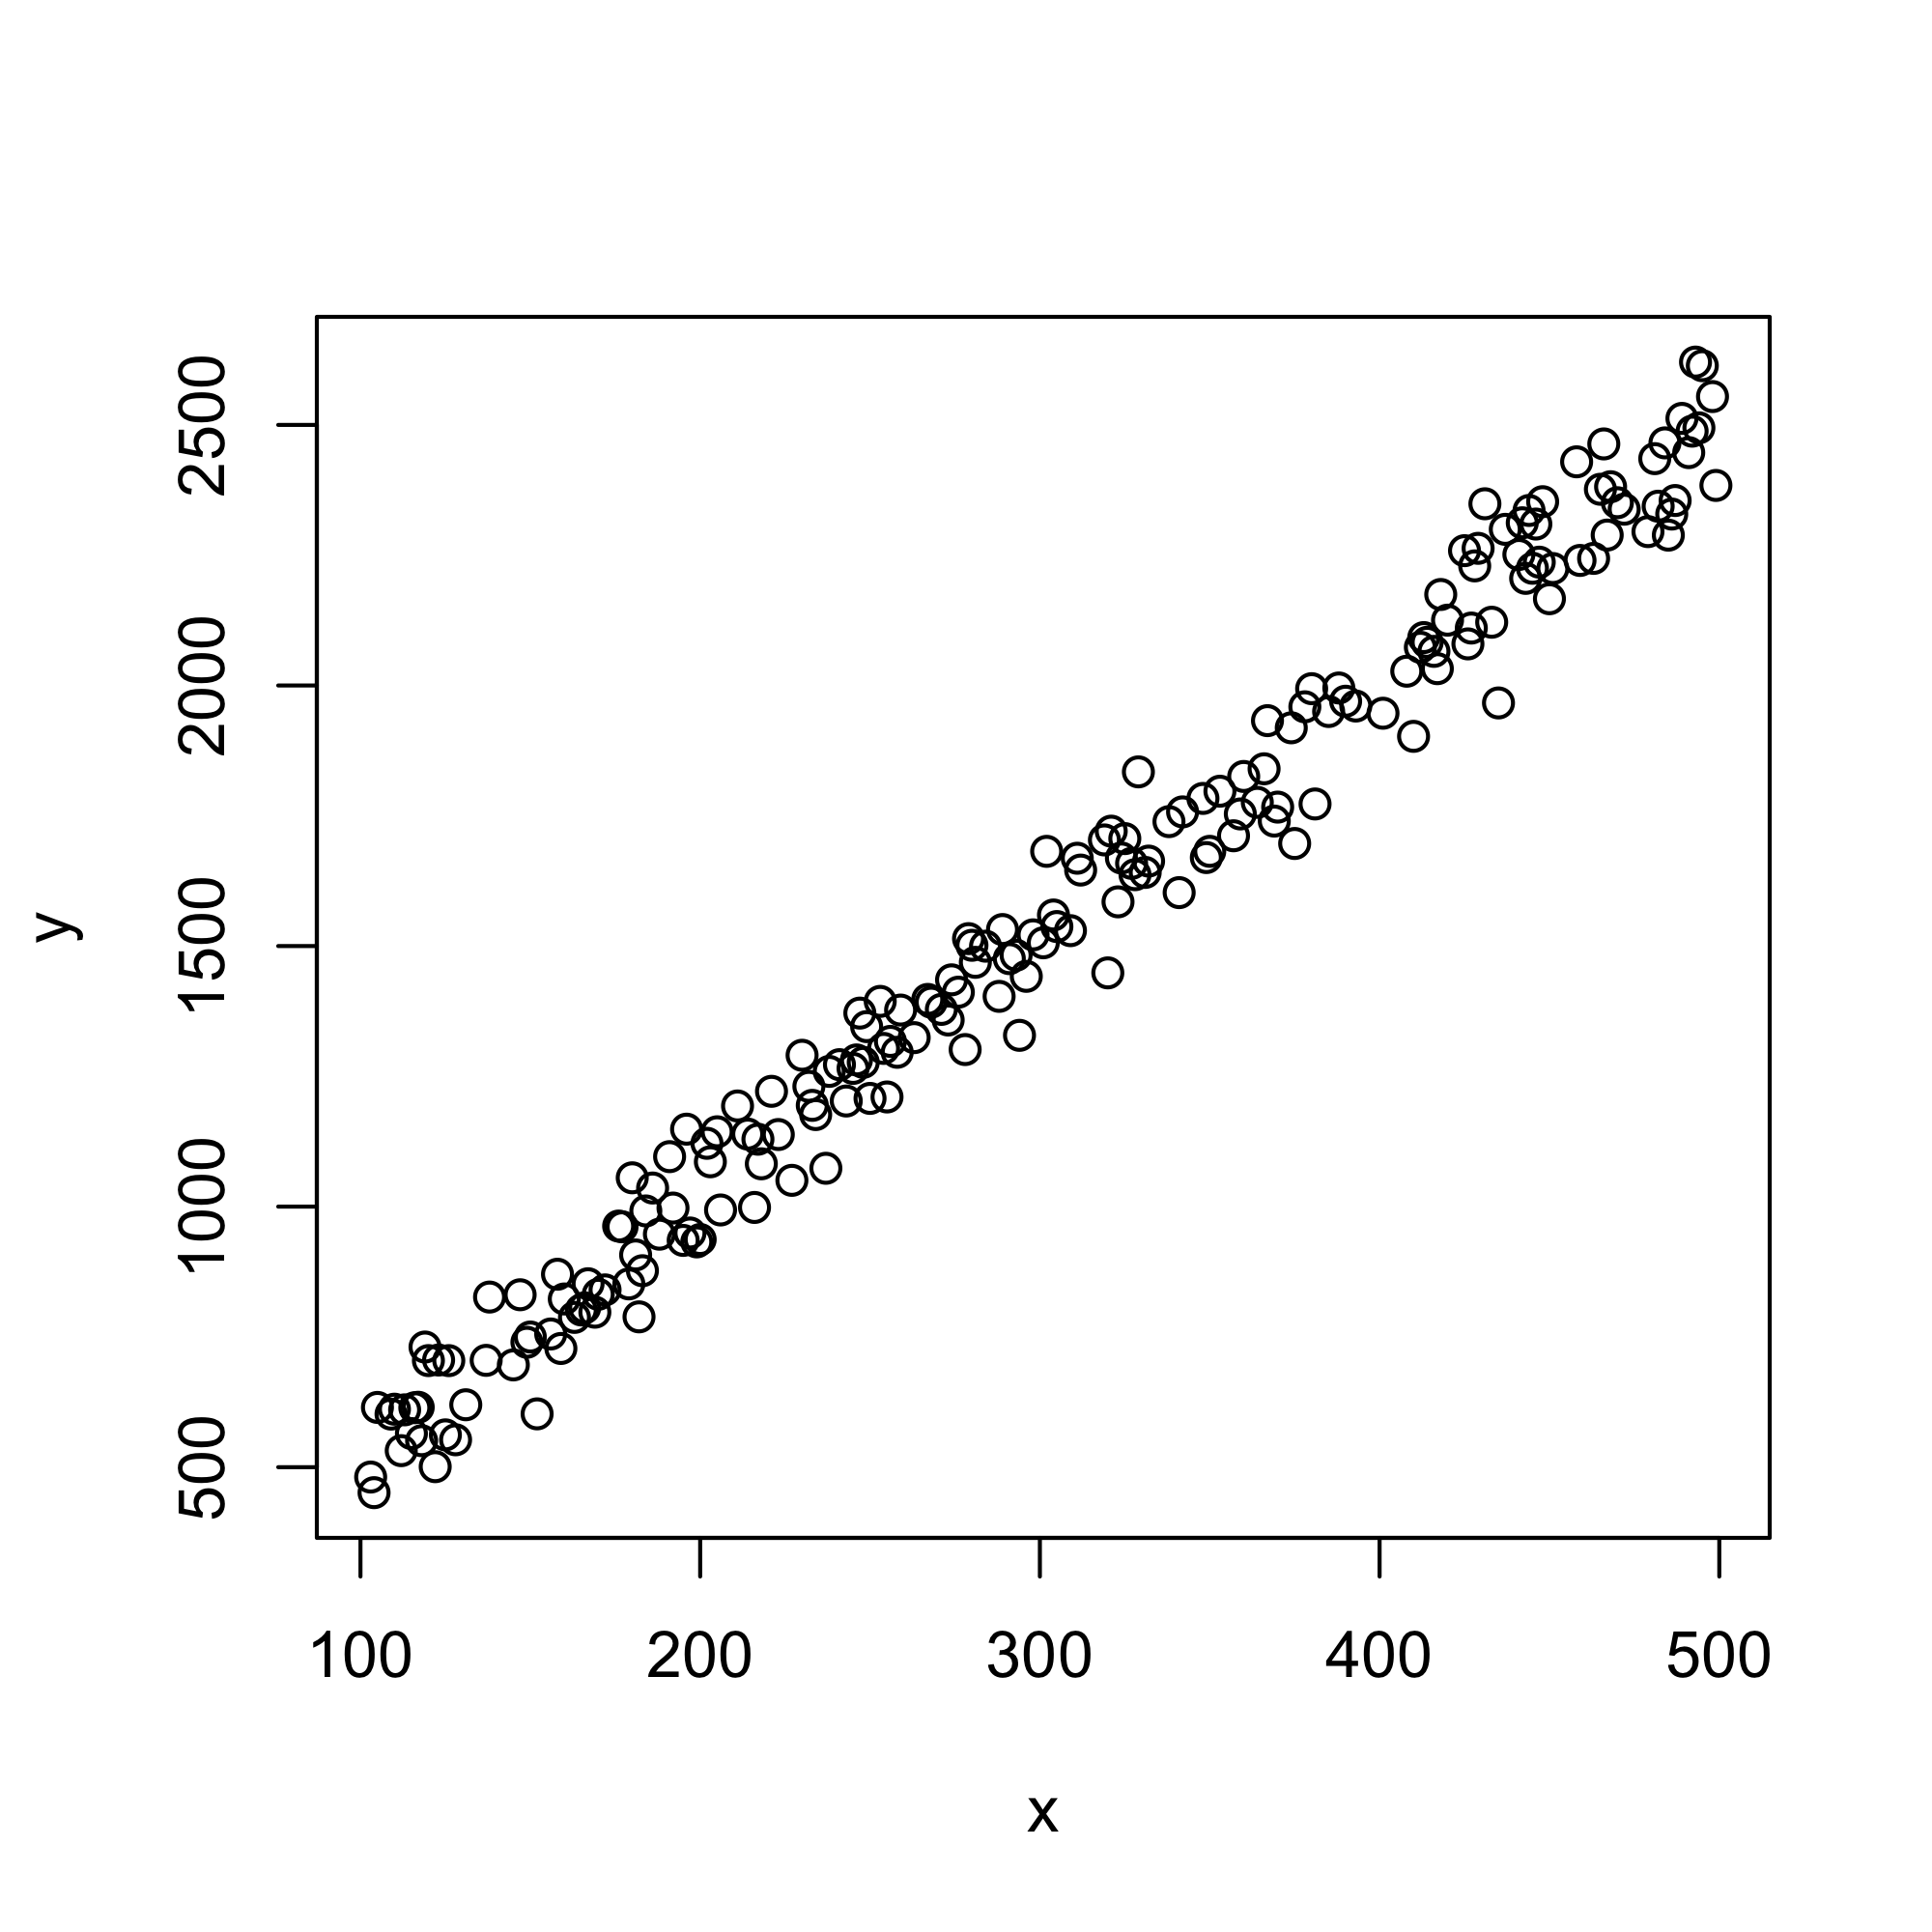
\includegraphics[width=\linewidth]{x-y1.png}
		\caption{$y = 5x+4+ N$.}
		\label{fig:xy_data_1}
	\end{subfigure}
	\hfill
	\begin{subfigure}{0.3\linewidth}
		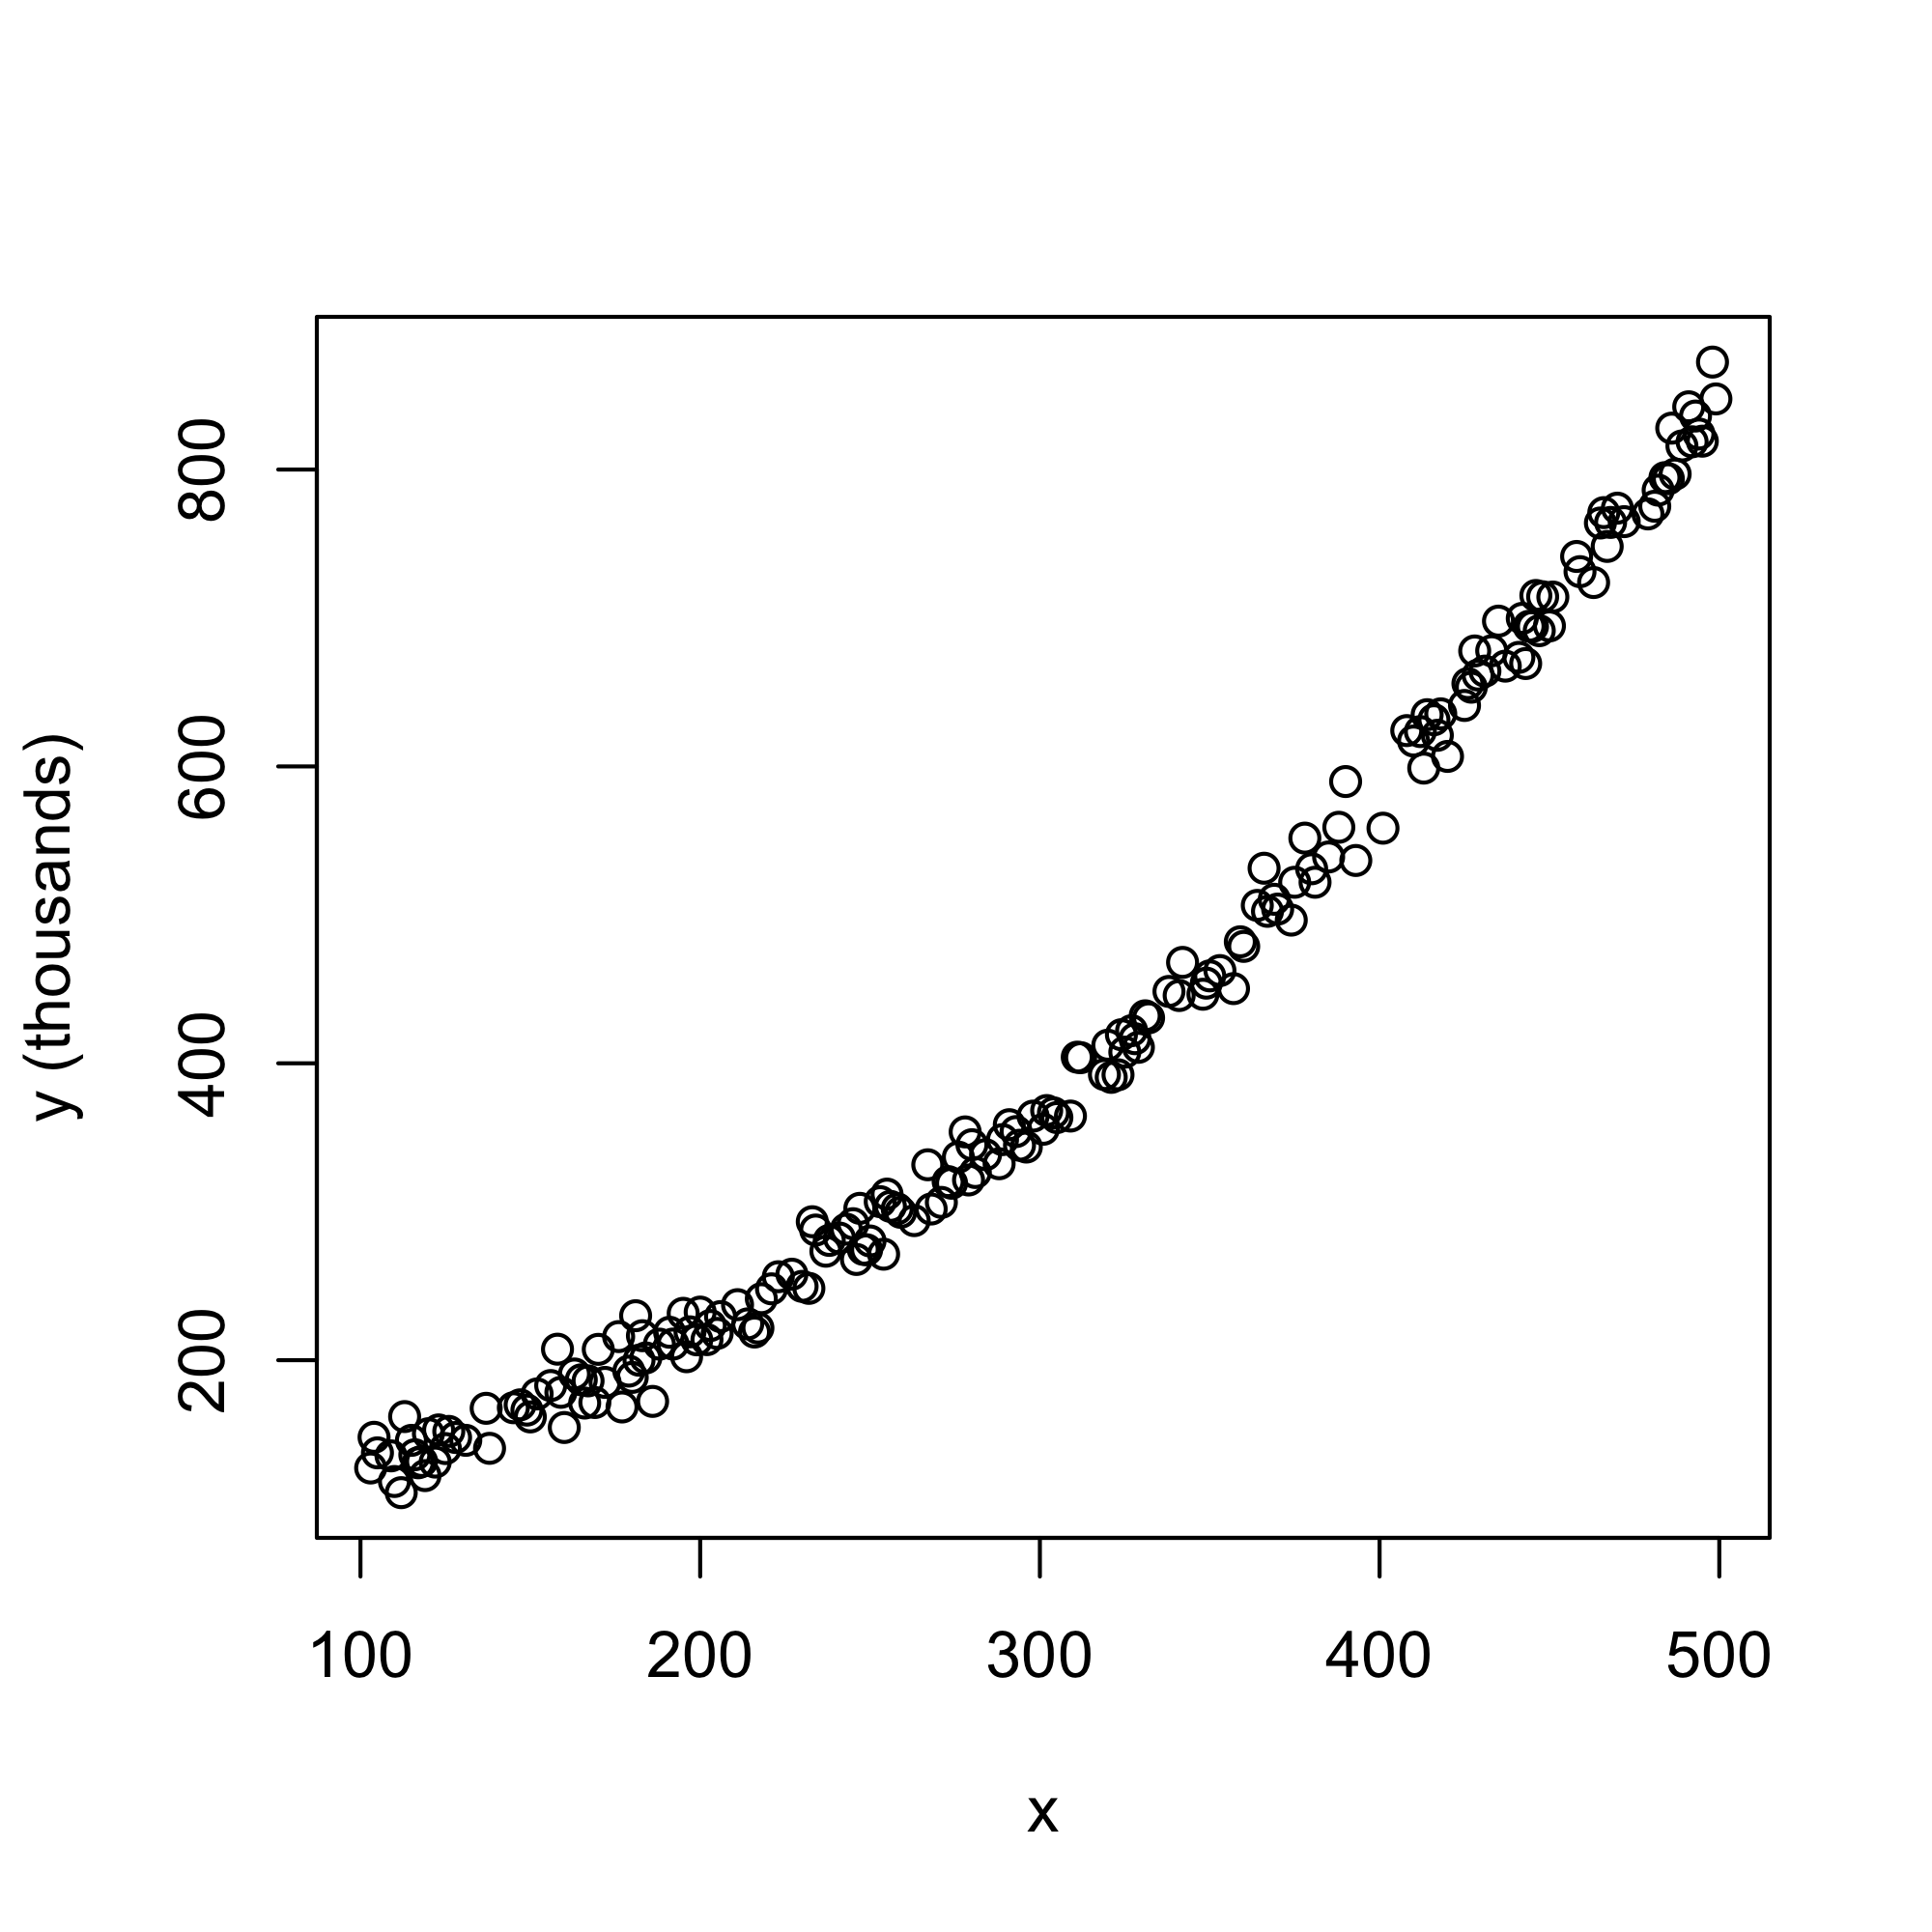
\includegraphics[width=\linewidth]{x-y2.png}
		\caption{$y = 3x^2 + 50 + N$.}
		\label{fig:xy_data_2}
	\end{subfigure}
	\hfill
	\begin{subfigure}{0.3\linewidth}
		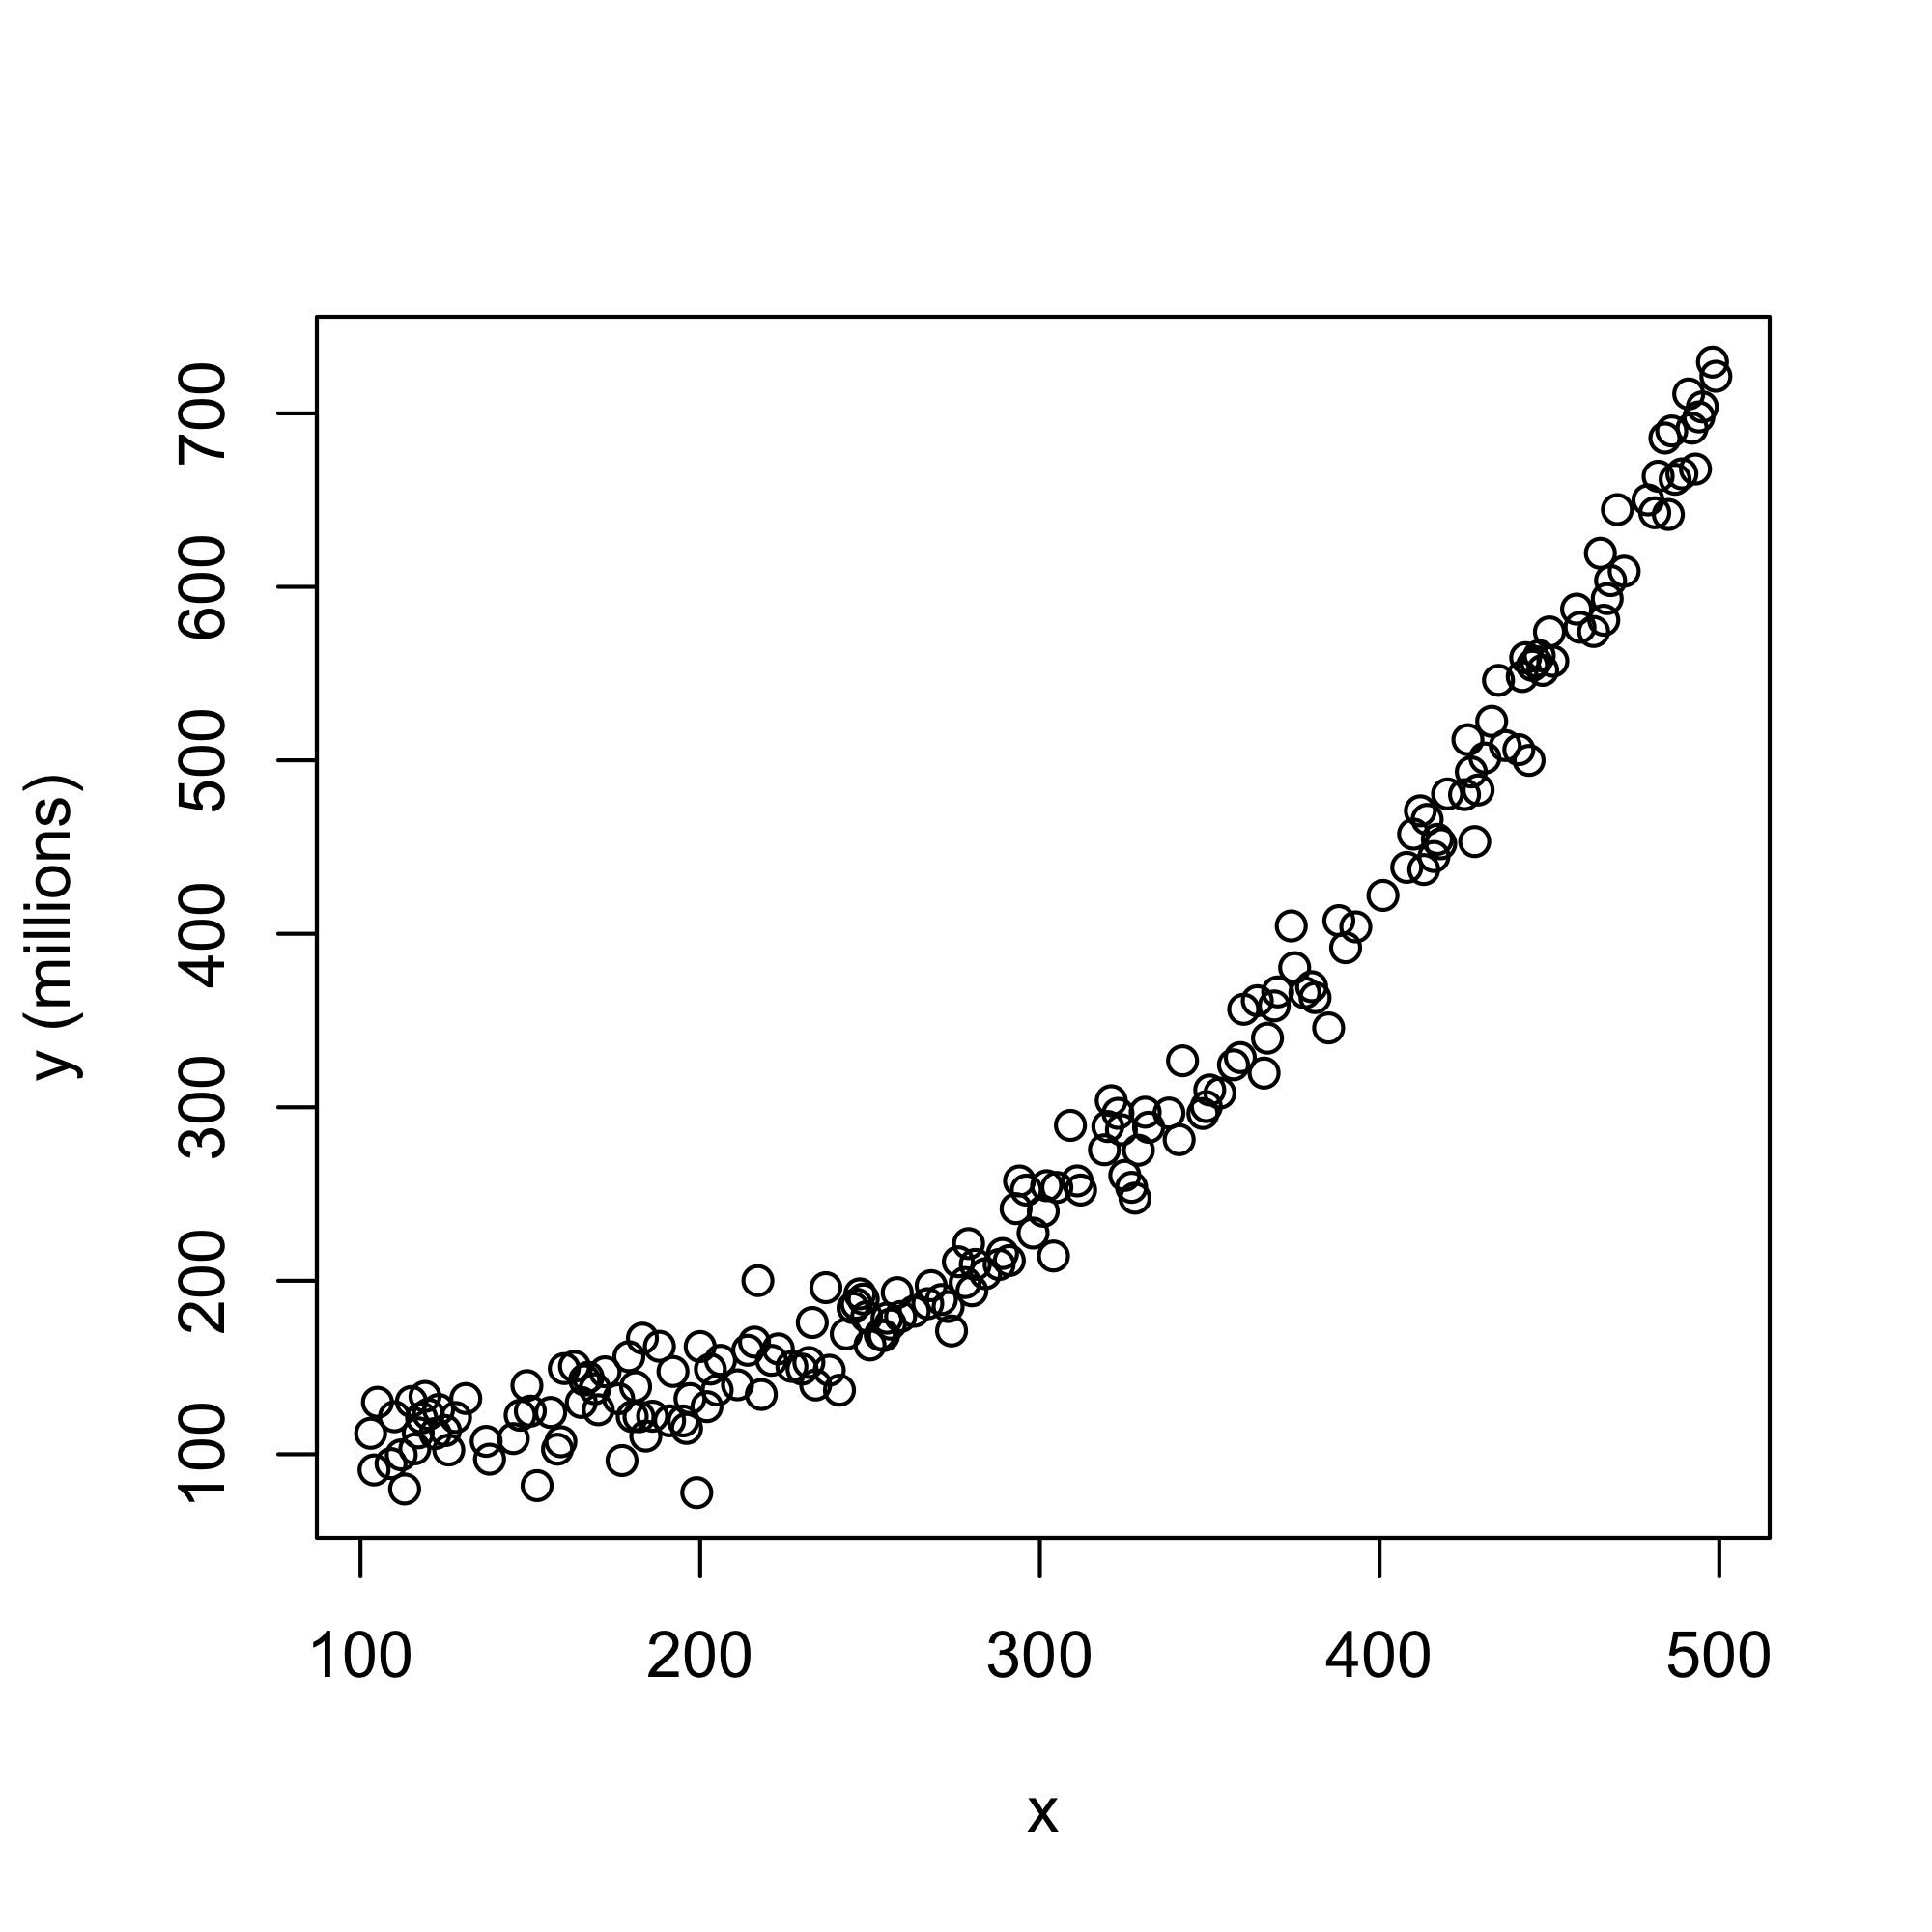
\includegraphics[width=\linewidth]{x-y3.png}
		\caption{$y = 5x^3 + .4 x^2 + 1 + N$.}
		\label{fig:xy_data_3}
	\end{subfigure}
	\begin{subfigure}{0.45\linewidth}
	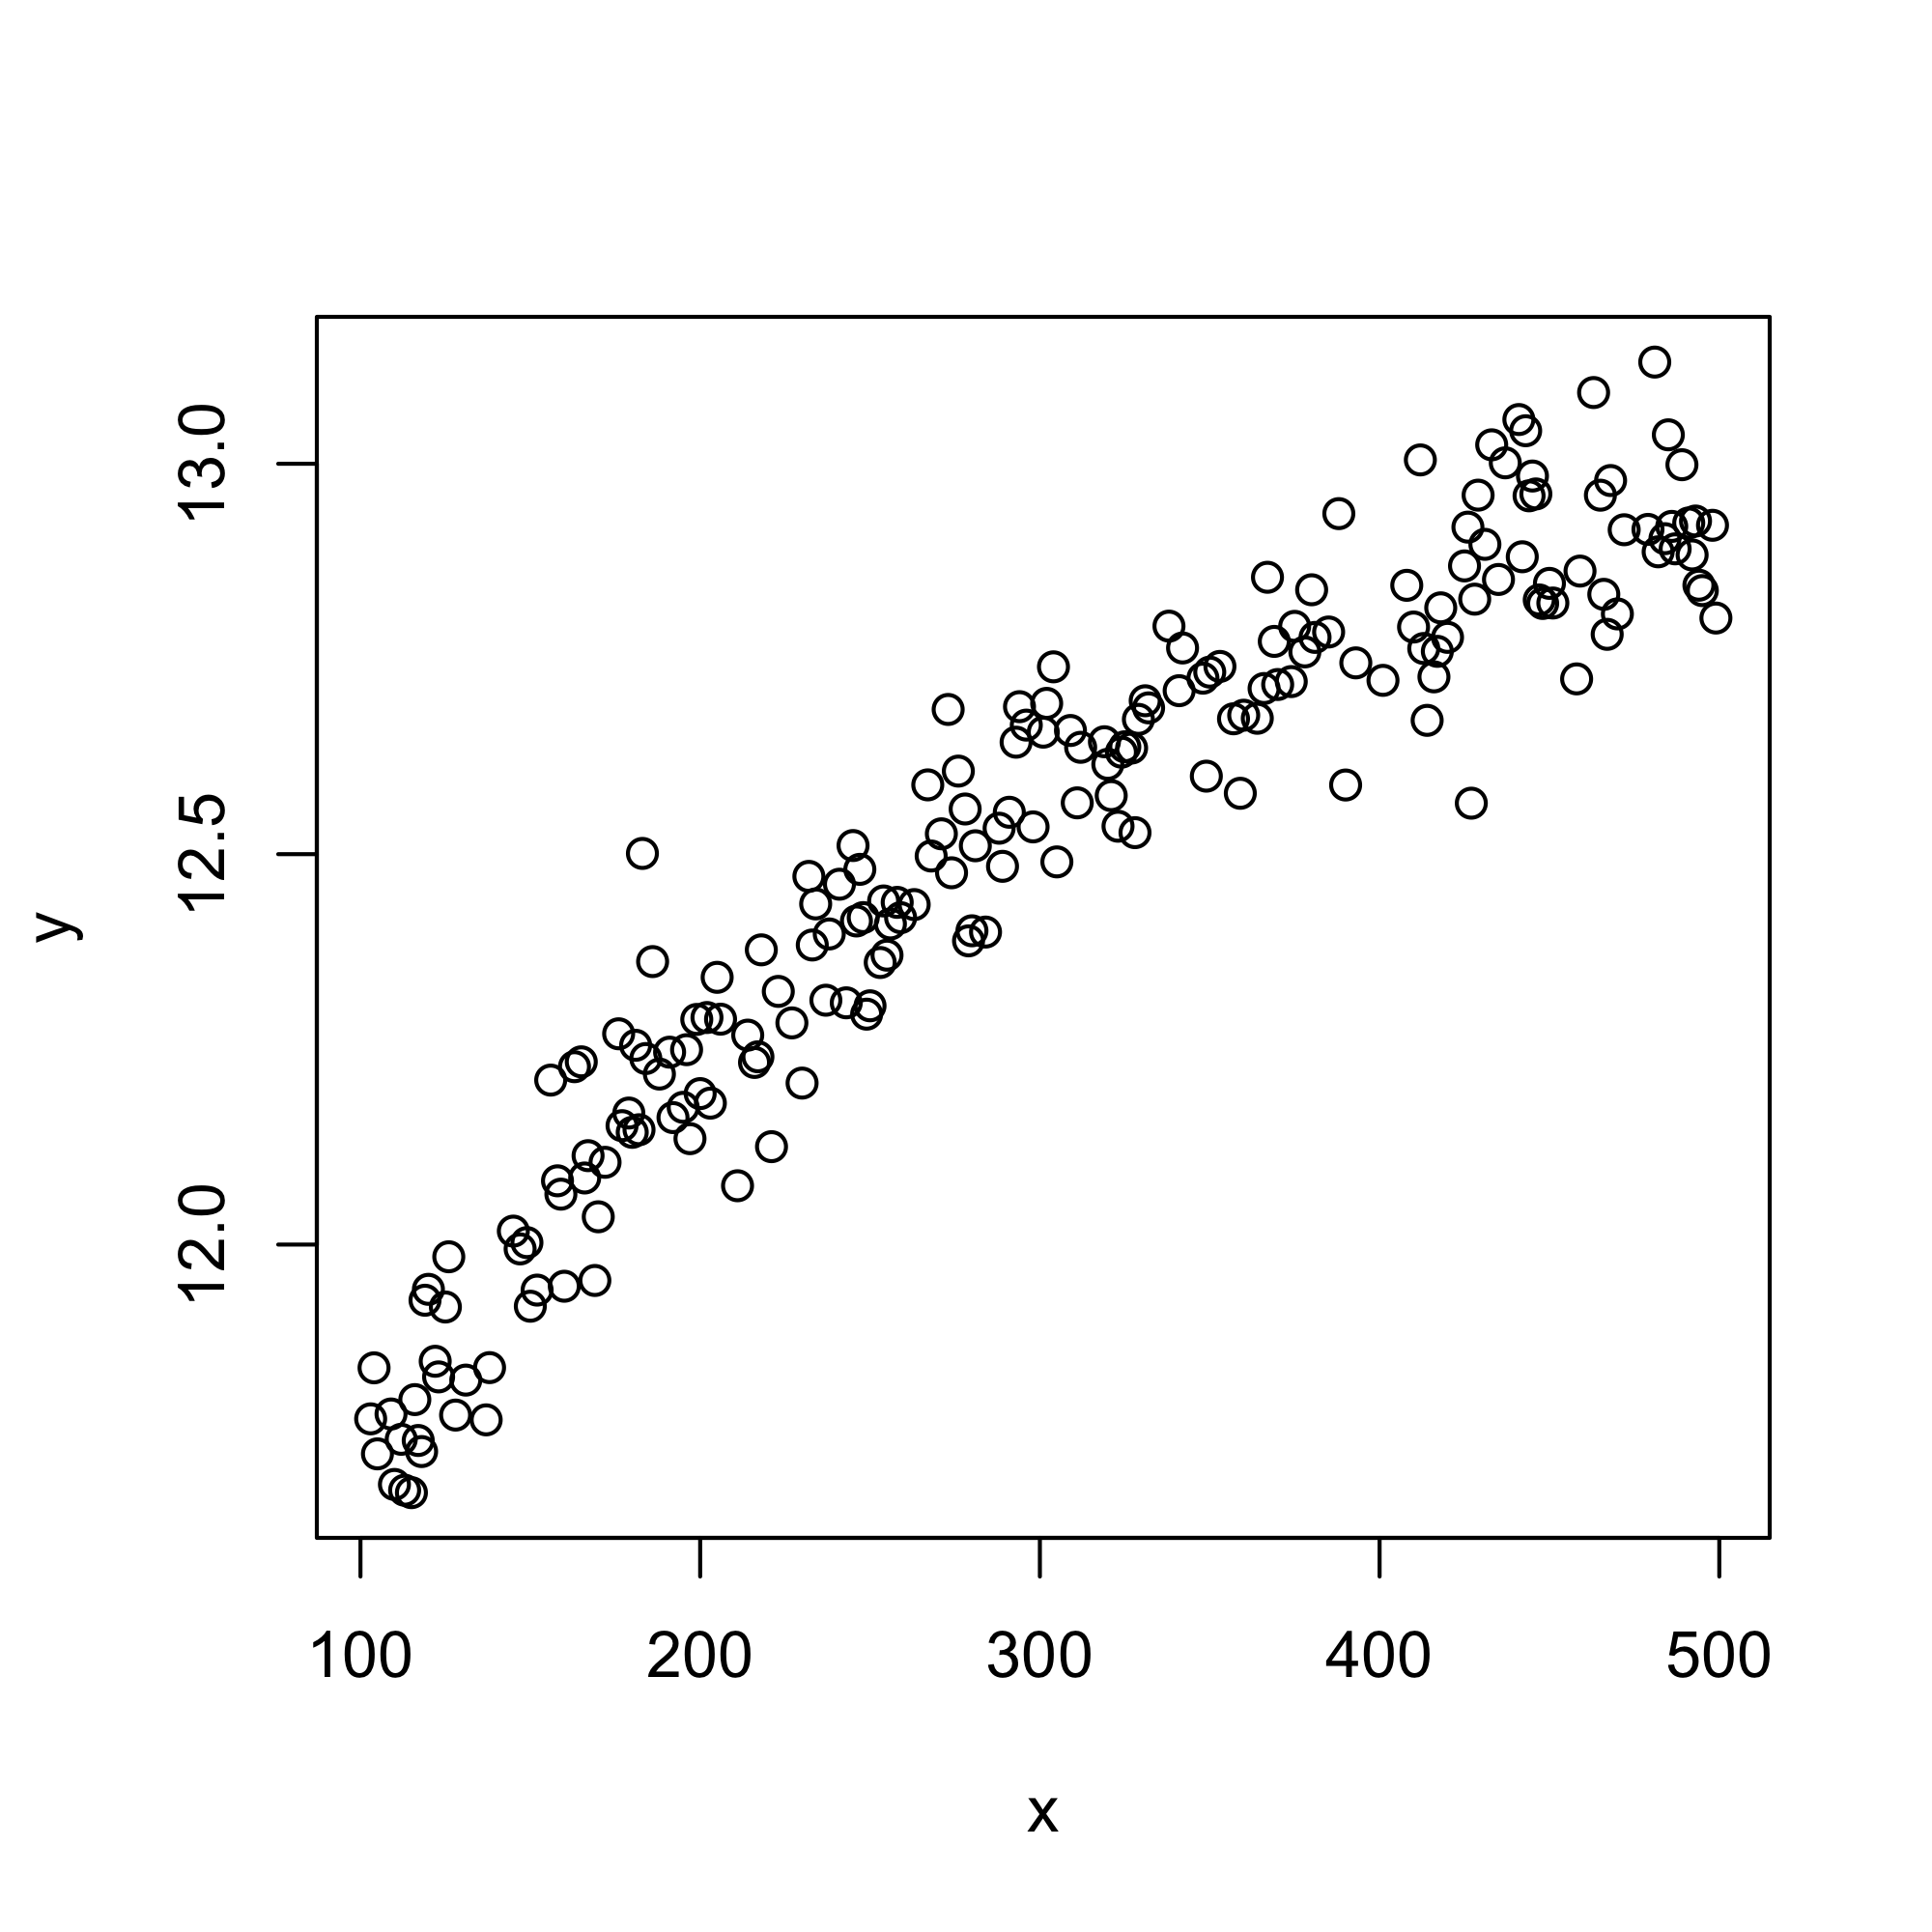
\includegraphics[width=\linewidth]{x-logy.png}
	\caption{$y = .8 \log(x) + 8 + N$.}
	\label{fig:xy_data_log}
	\end{subfigure}
	\hfill
	\begin{subfigure}{0.45\linewidth}
		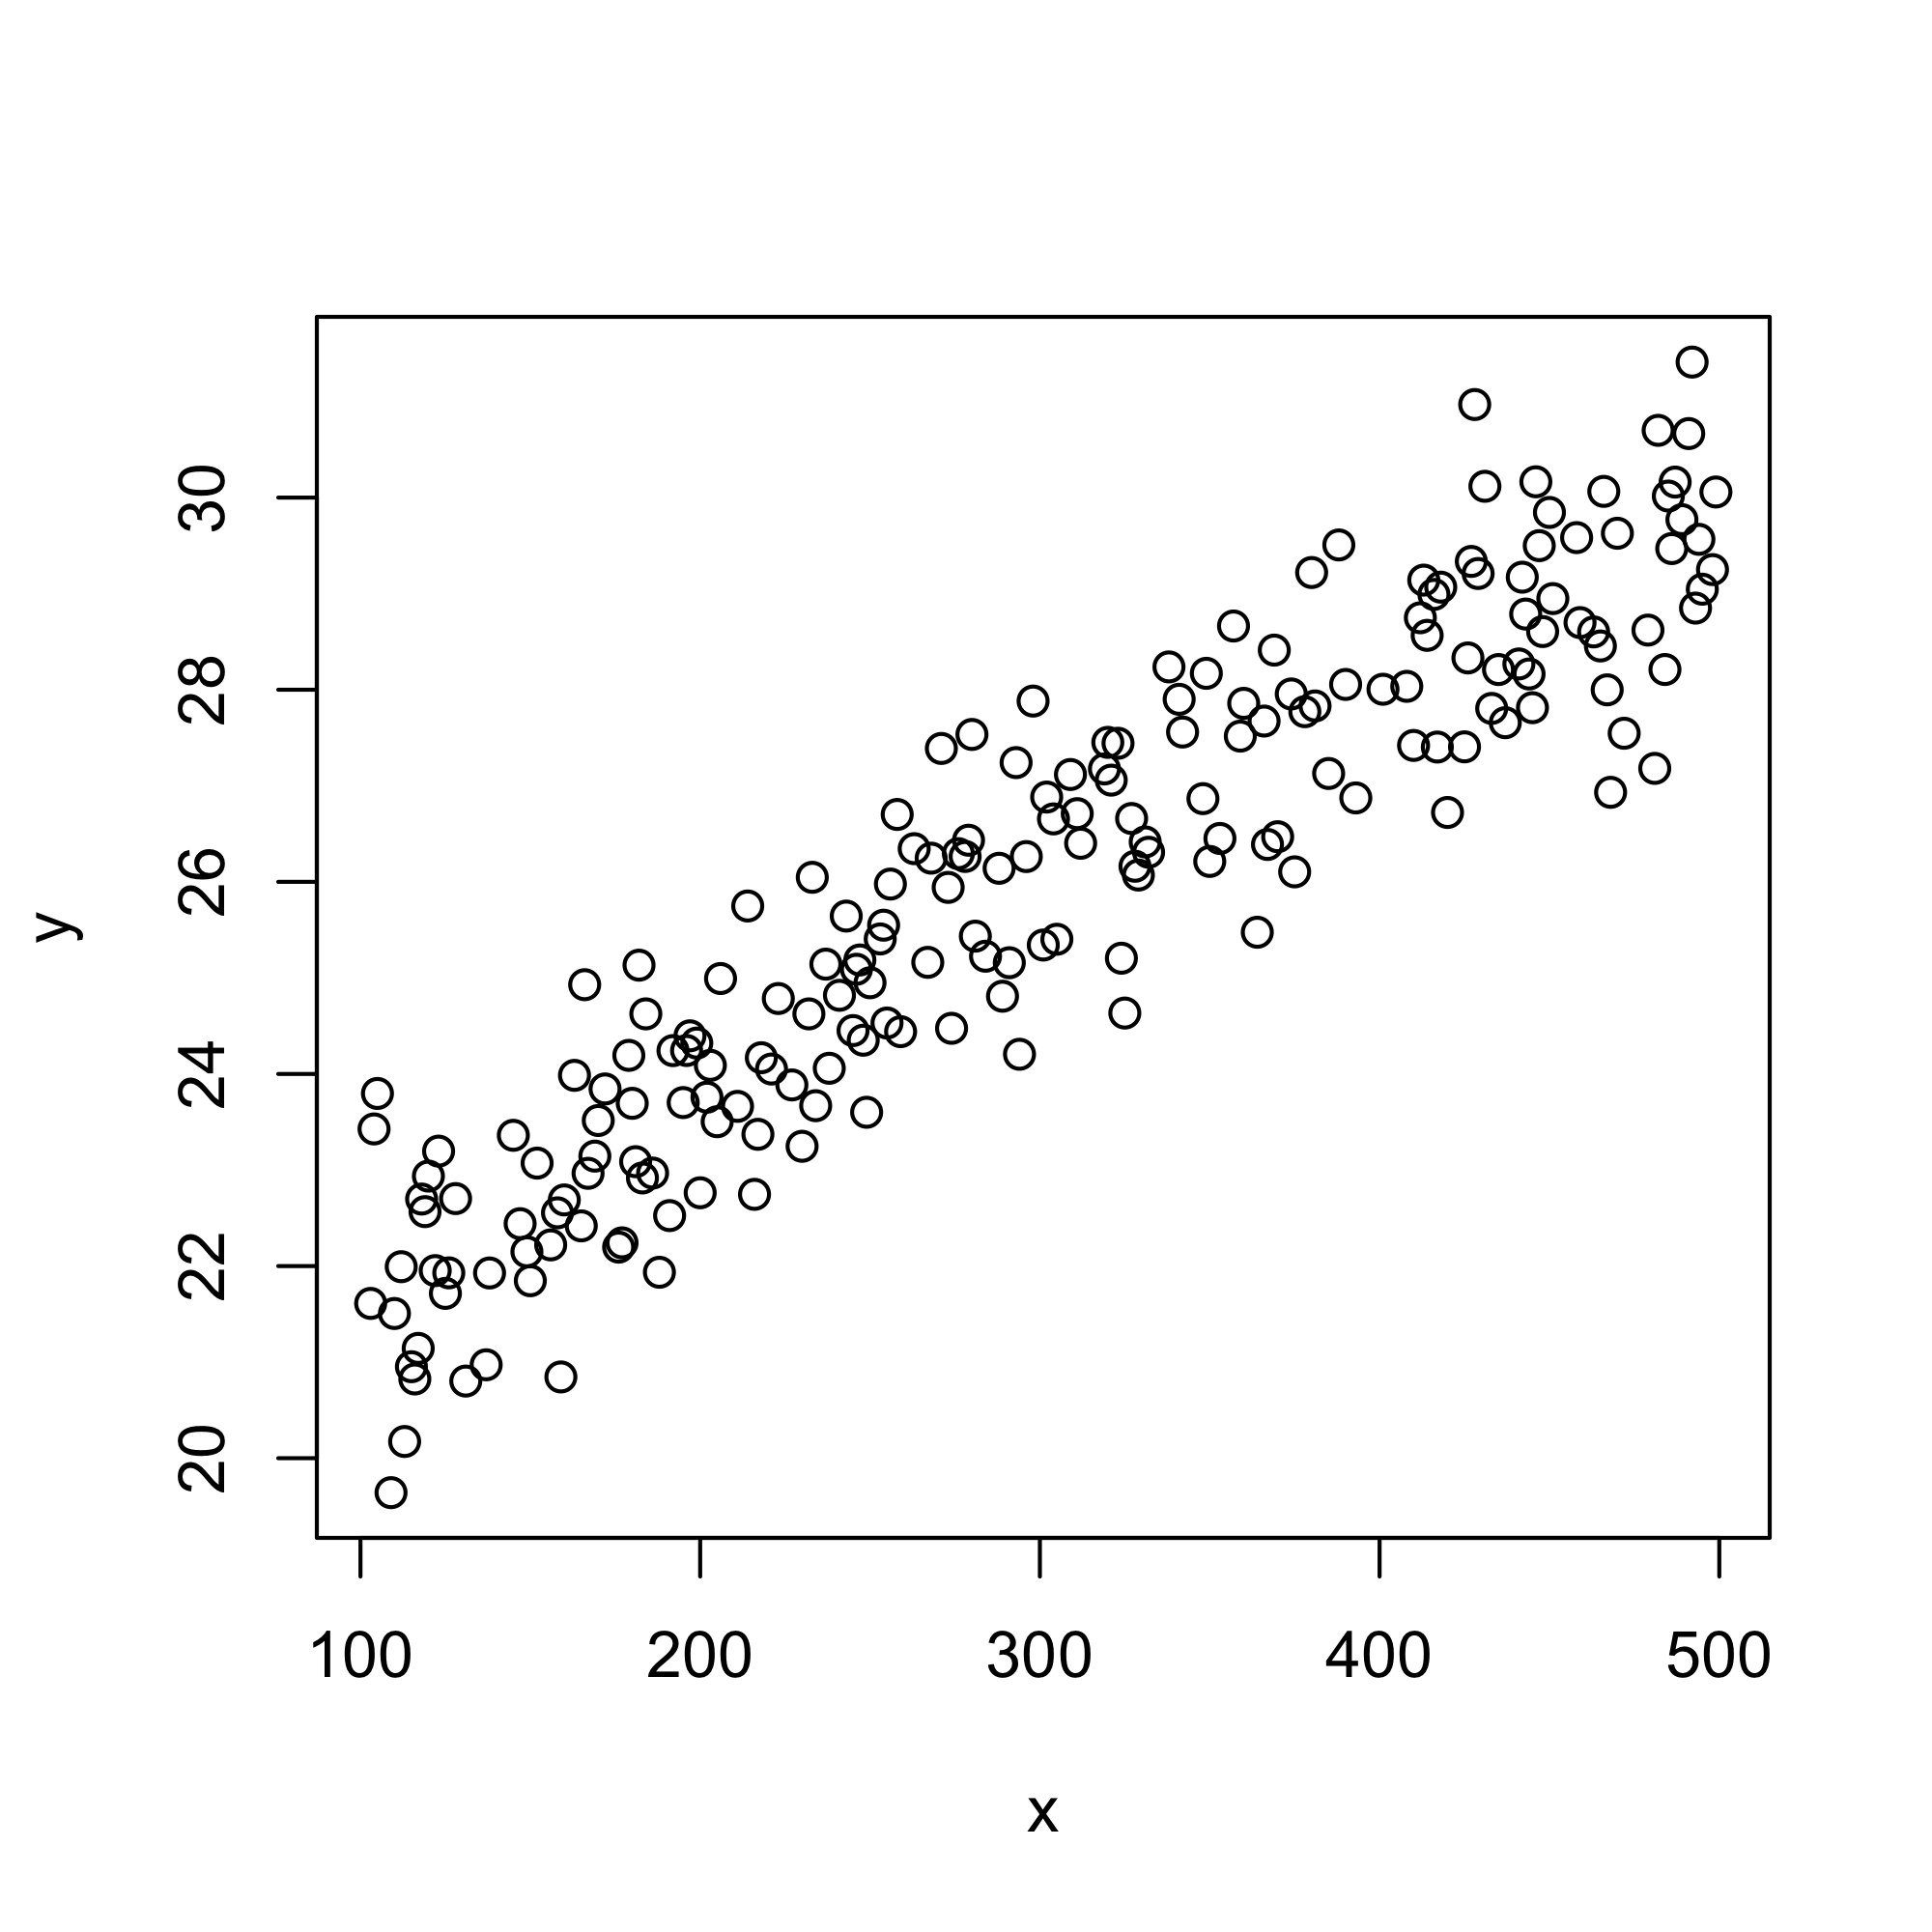
\includegraphics[width=\linewidth]{x-sqy.png}
		\caption{$y = .7 \sqrt{x} + 14 +N $.}
		\label{fig:xy_data_sq}
	\end{subfigure}
	\caption{Plots of the data generated.} 
	\label{fig:xy_data}
\end{figure}

For each of the $y$ values generated (see Table \ref{tab:xy_data}), the \texttt{choose\_lambda} function is used to obtain a $\lambda$ value, and the $y$ values are transformed. Then, using R's \texttt{lm} function, a linear regression is performed on the $x, \tilde{y}_\lambda$ values, which gives a linear function $\tilde{y}_\lambda = a x + b$.  Finally, an inverse transformation is applied to get a function $y = f(x)$ fitting the original values. The results of this process are plotted in Figure \ref{fig:fits_xy}.

\begin{figure}
	\centering
	\begin{subfigure}{0.3\linewidth}
		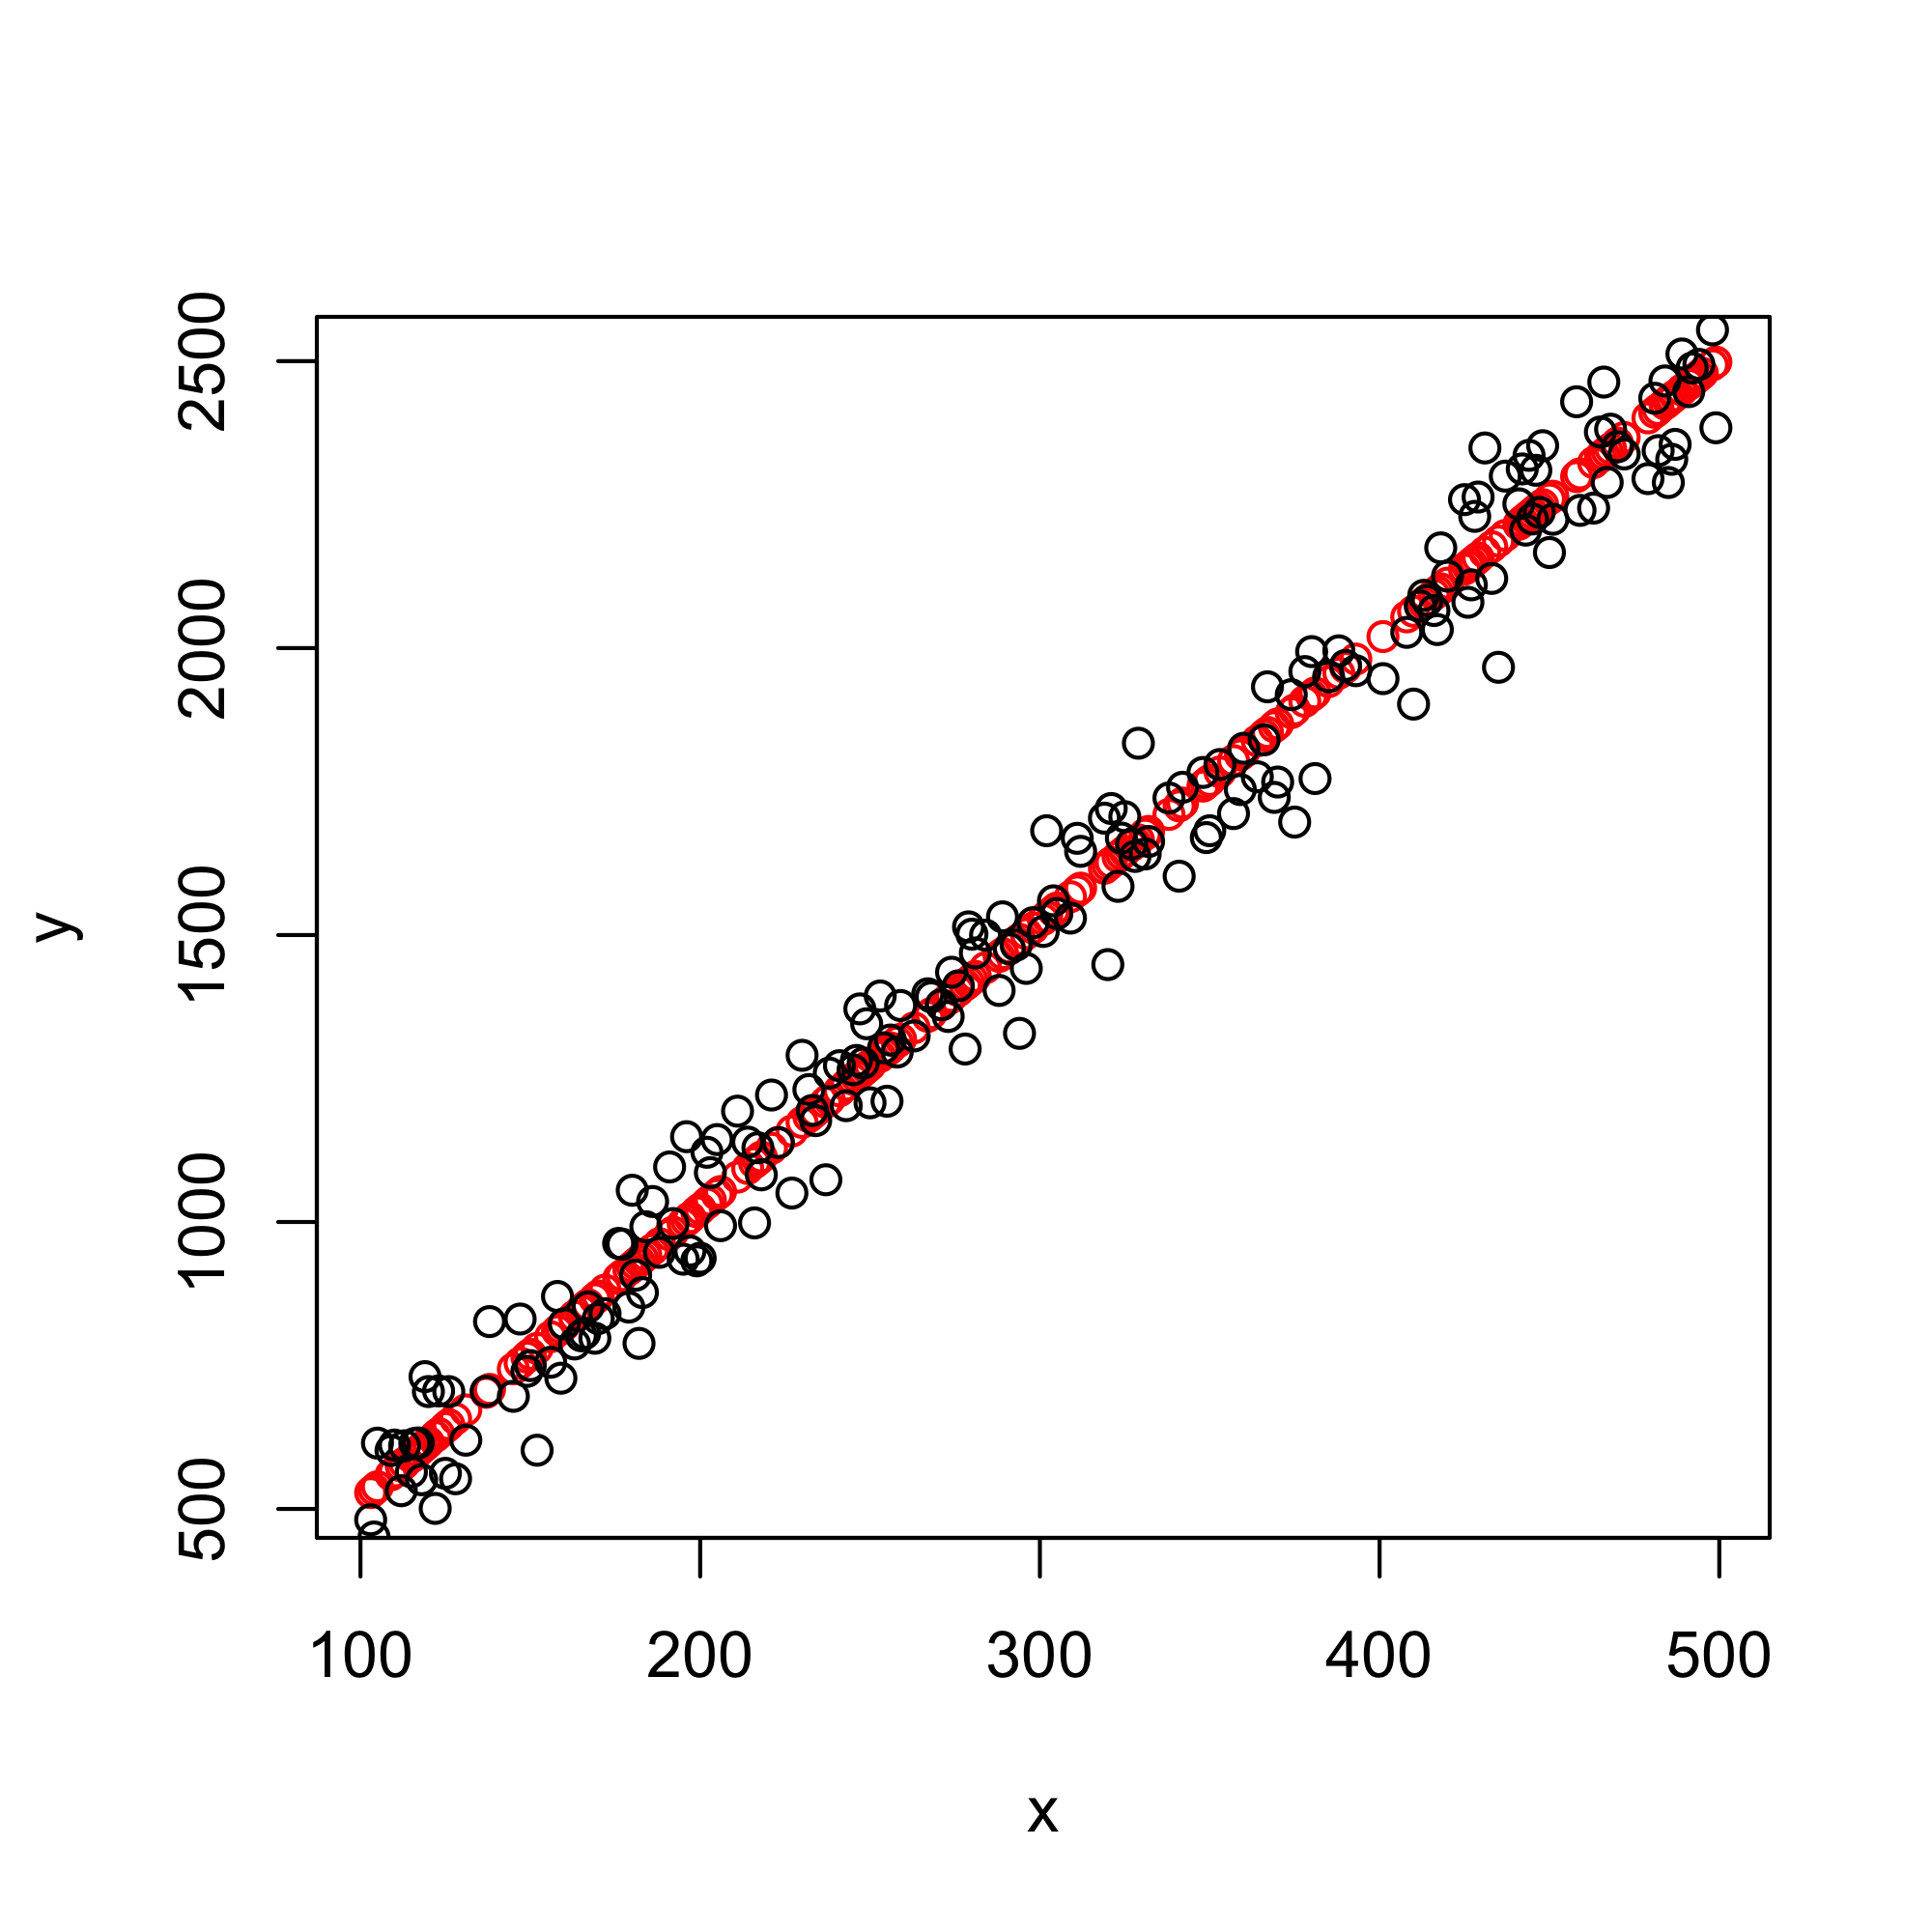
\includegraphics[width=\linewidth]{fit_x_y1.png}
		\caption{In black, $y = 5x+4+ N$, and in red, a curve fitted with $\lambda = 1.04$.}
		\label{fig:fits_xy_1}
	\end{subfigure}
	\hfill
	\begin{subfigure}{0.3\linewidth}
		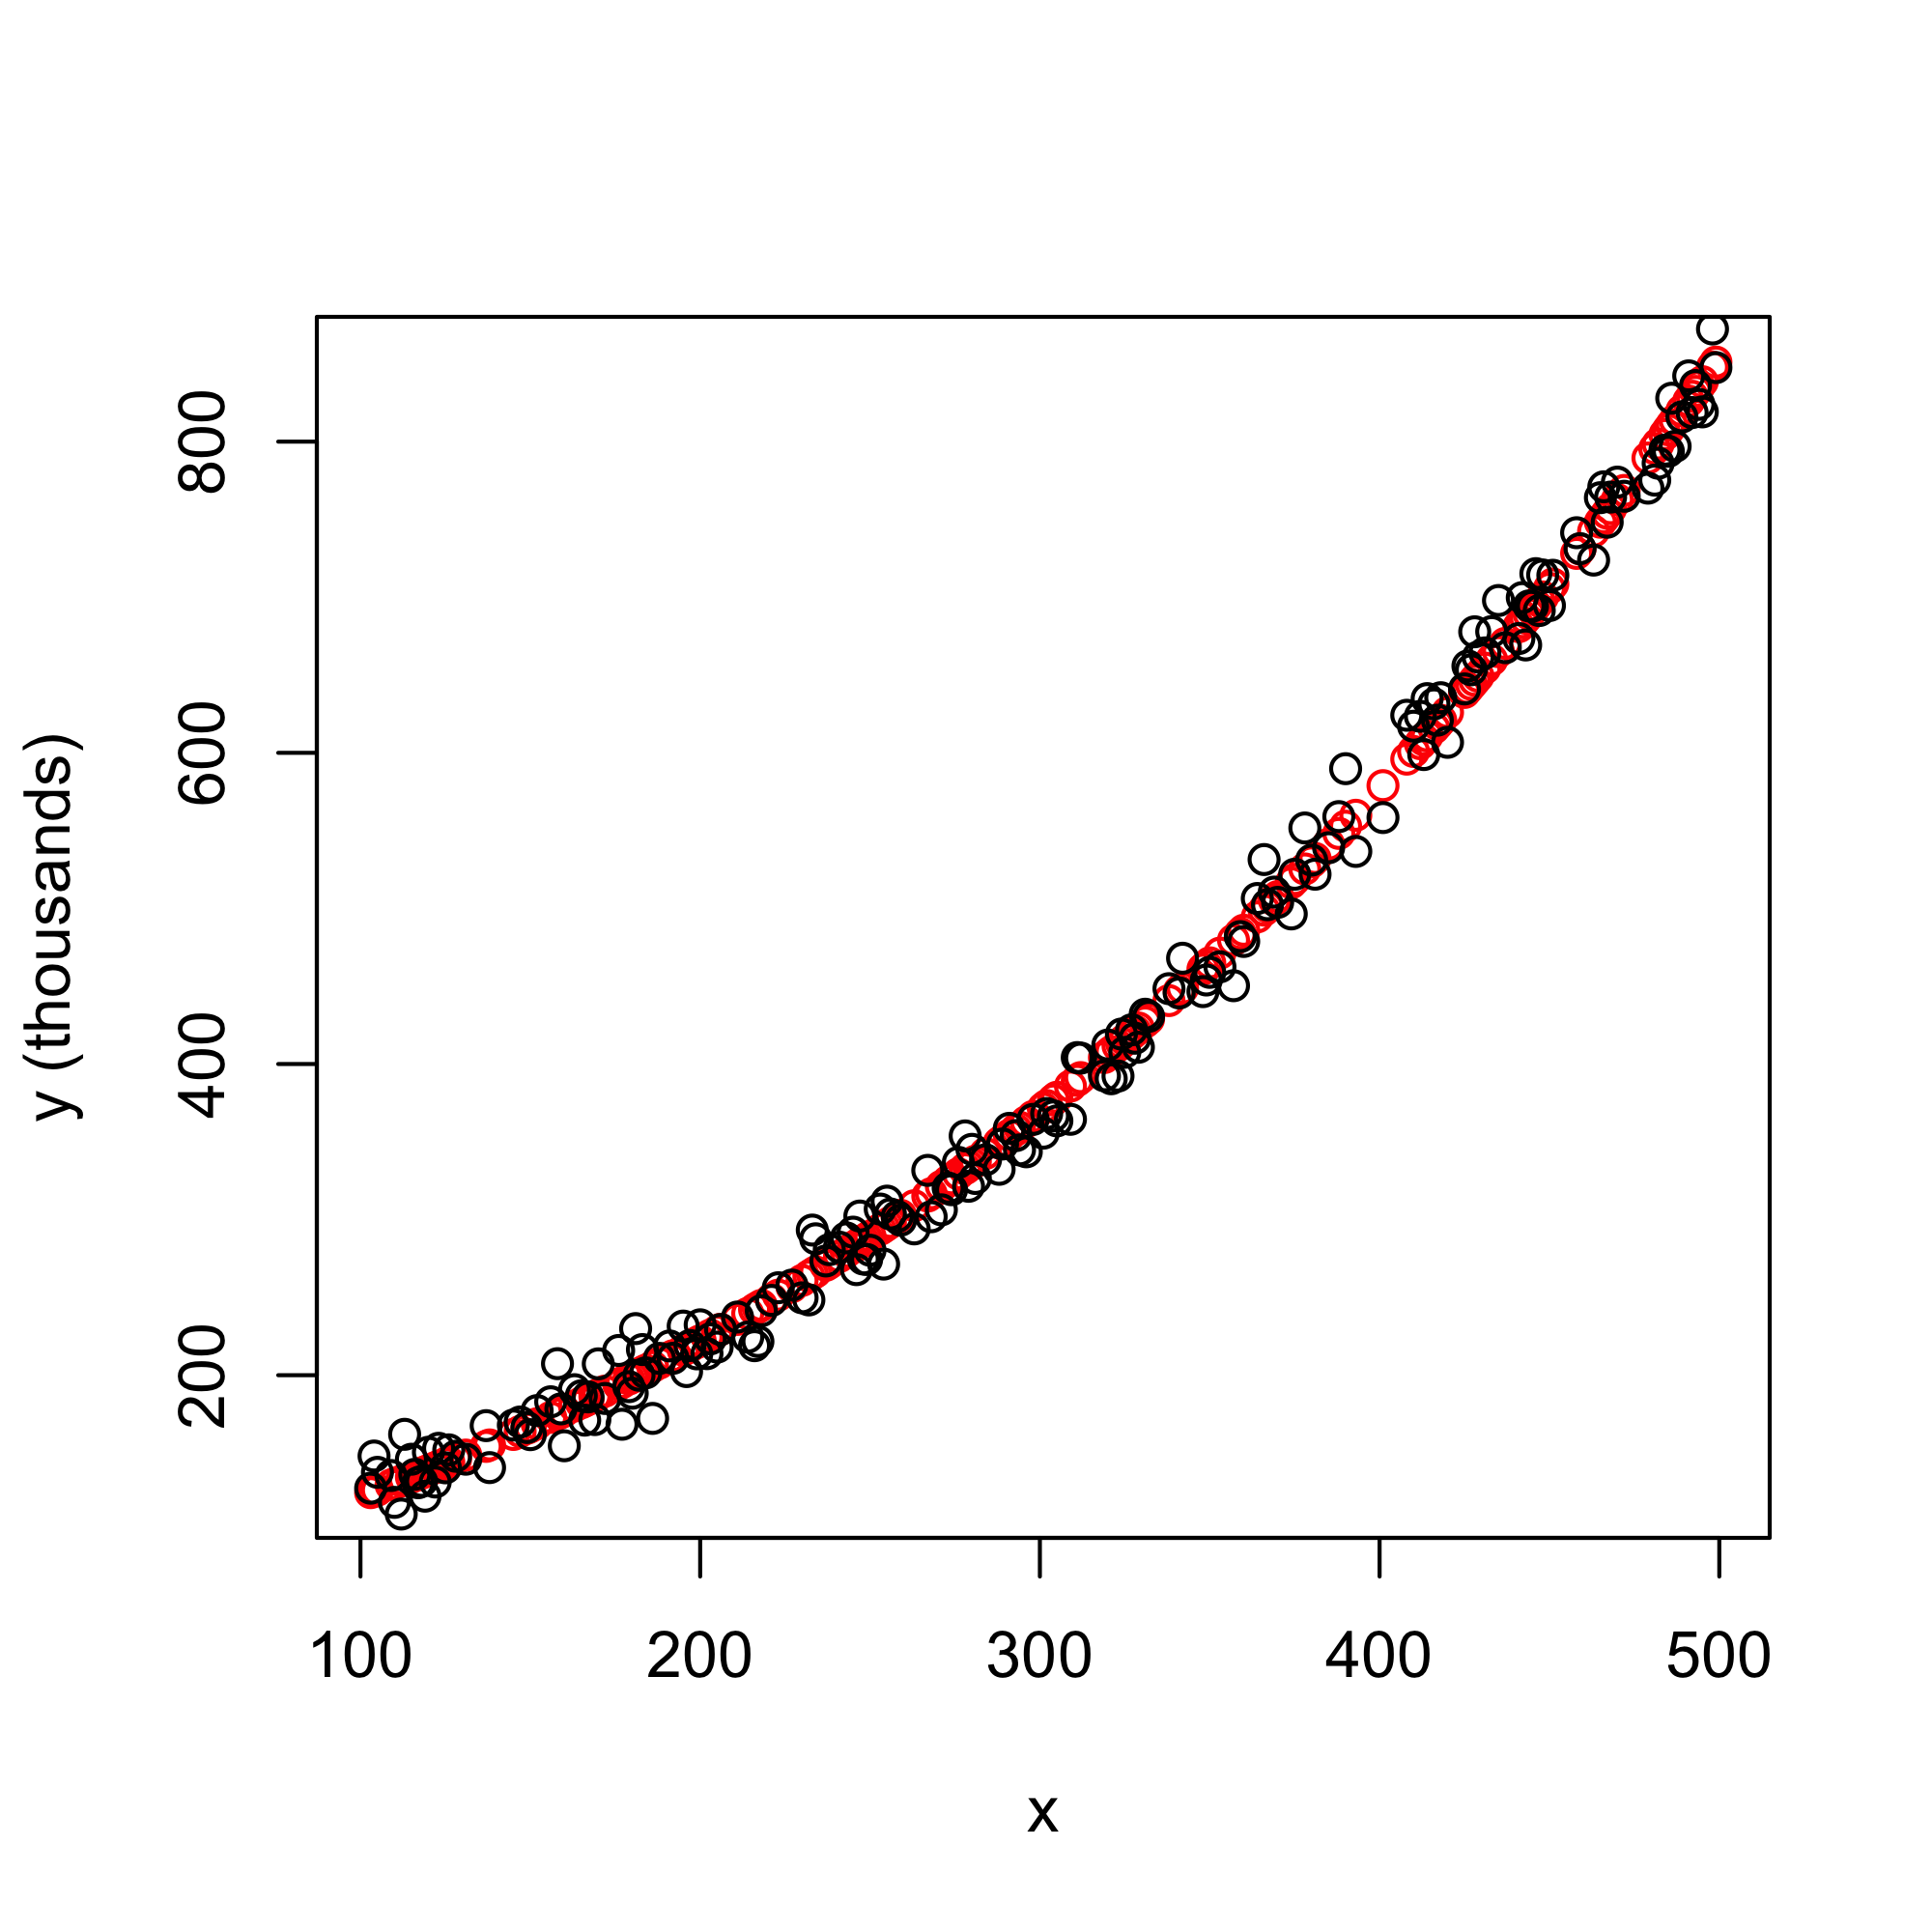
\includegraphics[width=\linewidth]{fit_x_y2.png}
		\caption{In black, $y = 3x^2 + 50 + N$, and in red, a curve fitted with $\lambda = 0.29$.}
		\label{fig:fits_xy_2}
	\end{subfigure}
	\hfill
	\begin{subfigure}{0.3\linewidth}
		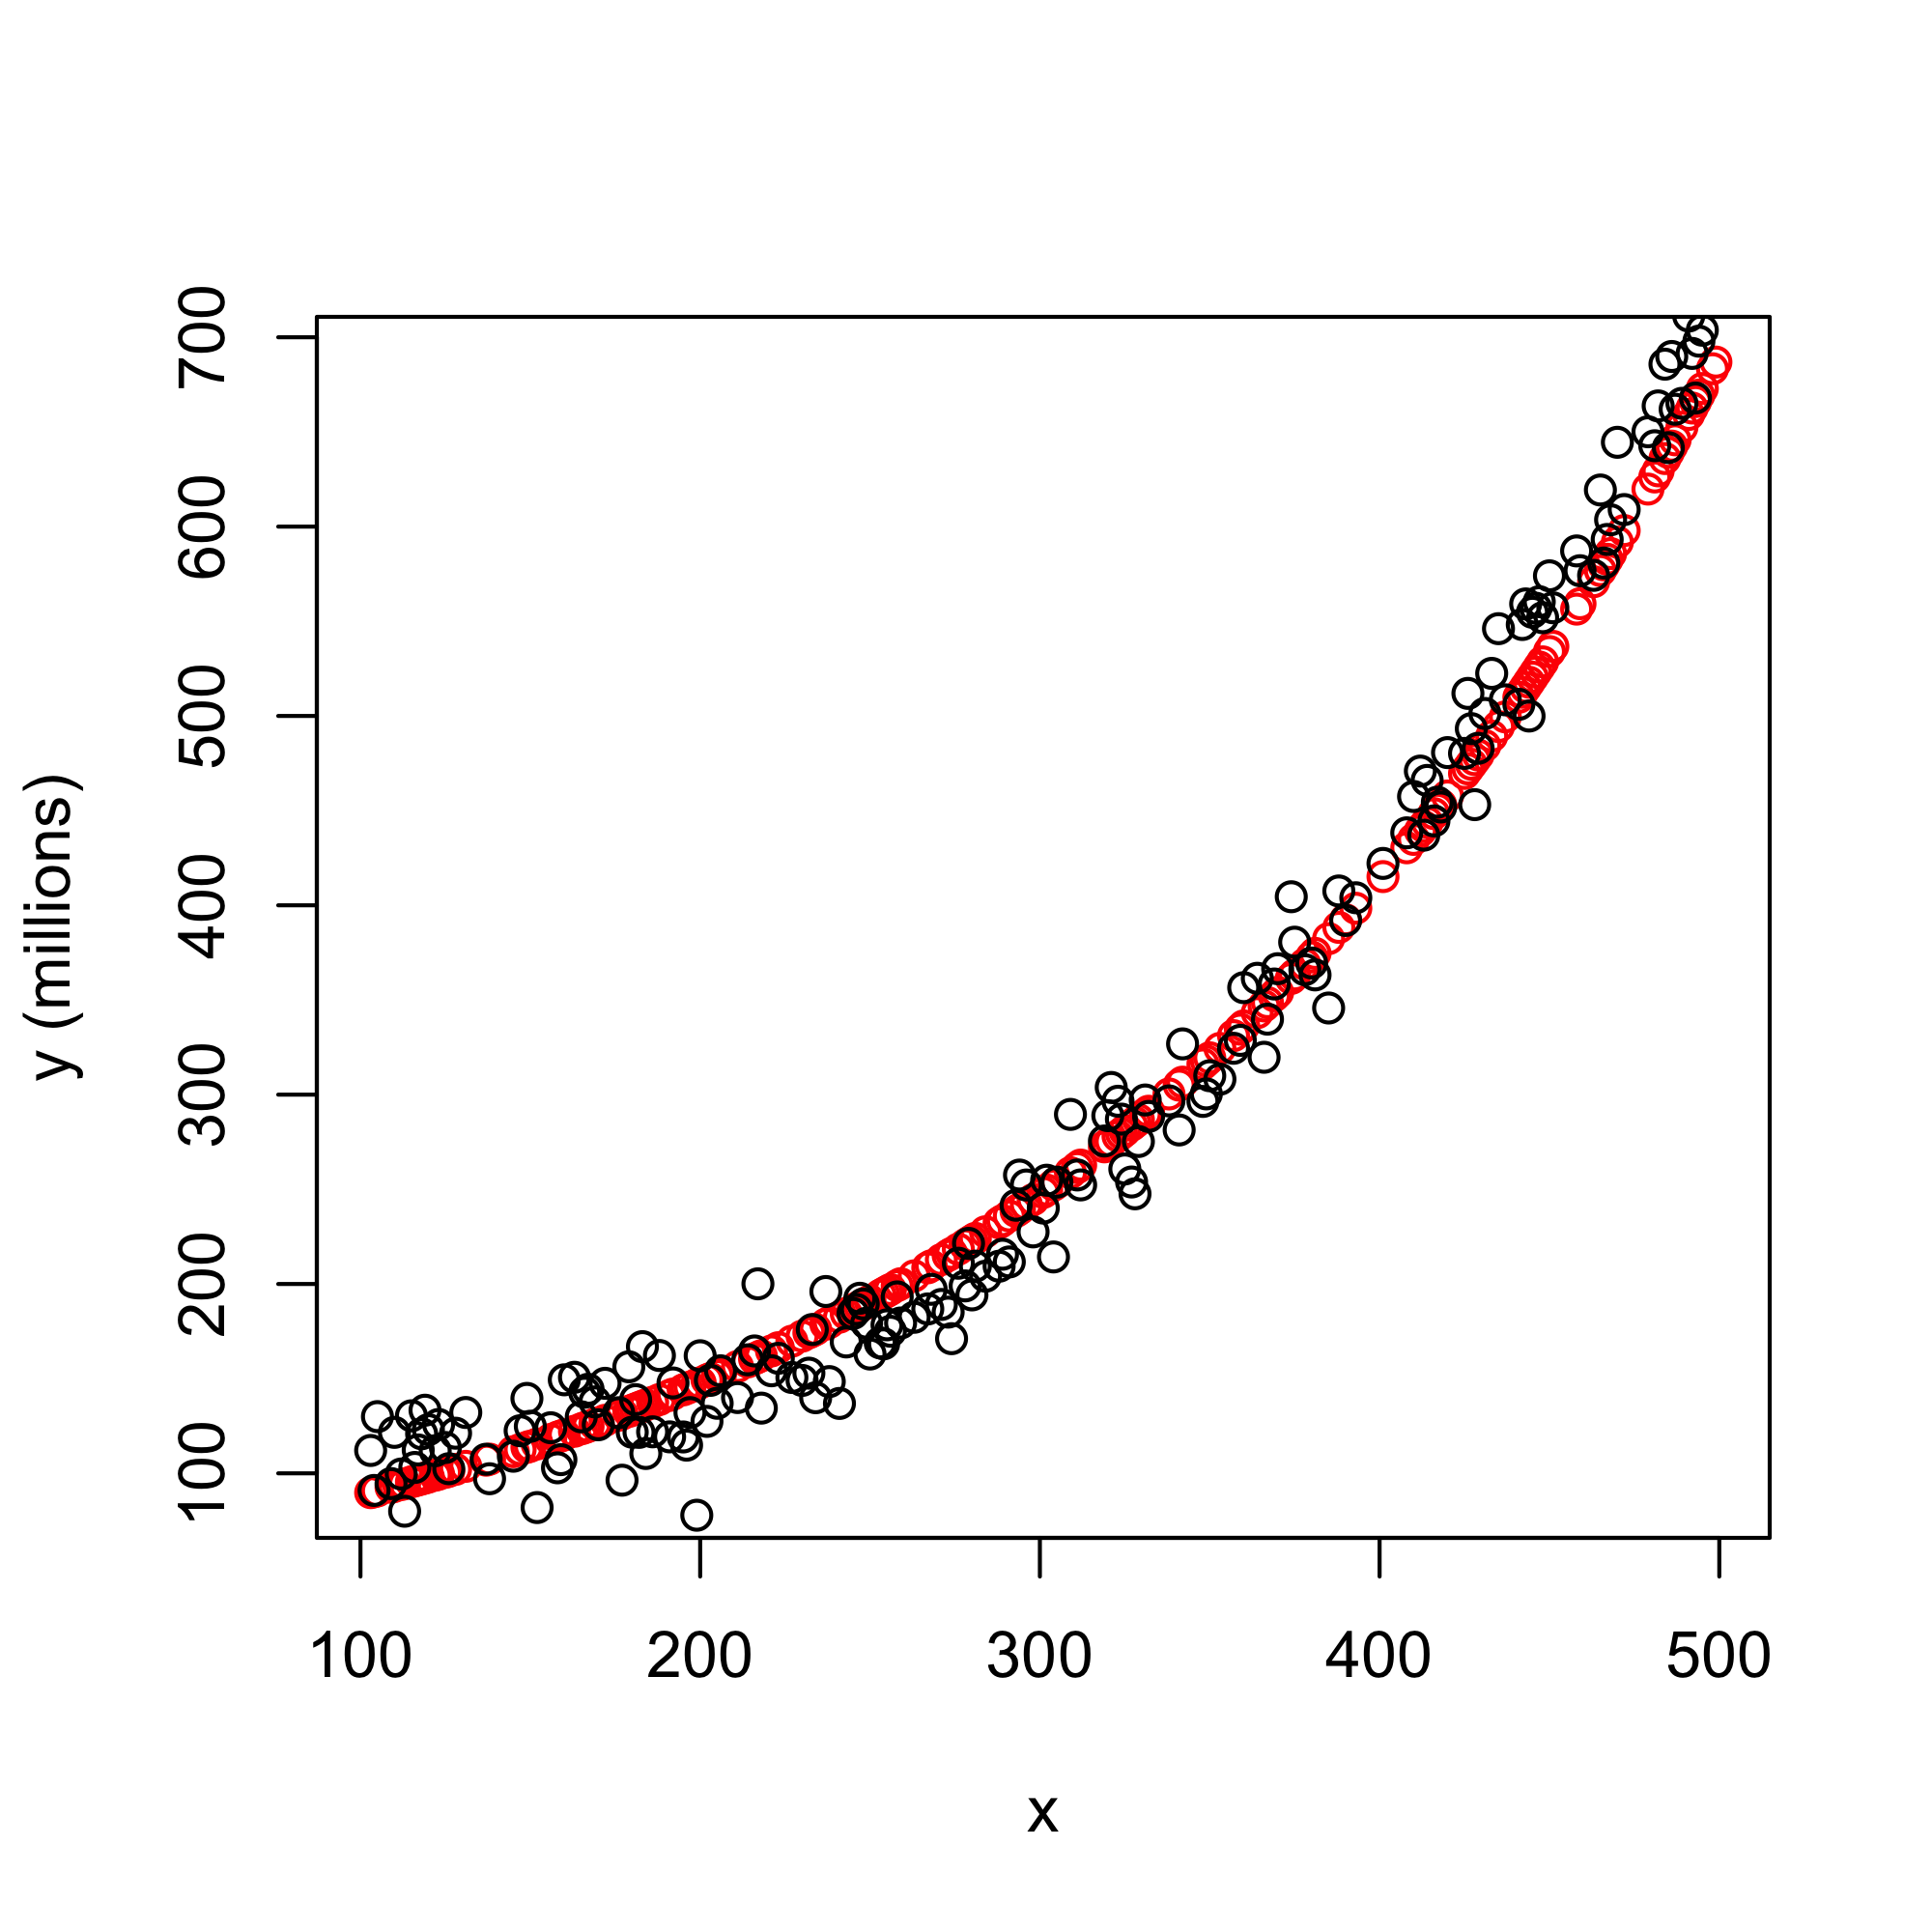
\includegraphics[width=\linewidth]{fit_x_y3.png}
    	\caption{In black, $y = 5x^3 + .4 x^2 + 1 + N$, and in red, a curve fitted with $\lambda = 0$.}
		\label{fig:fits_xy_3}
	\end{subfigure}
	\begin{subfigure}{0.45\linewidth}
		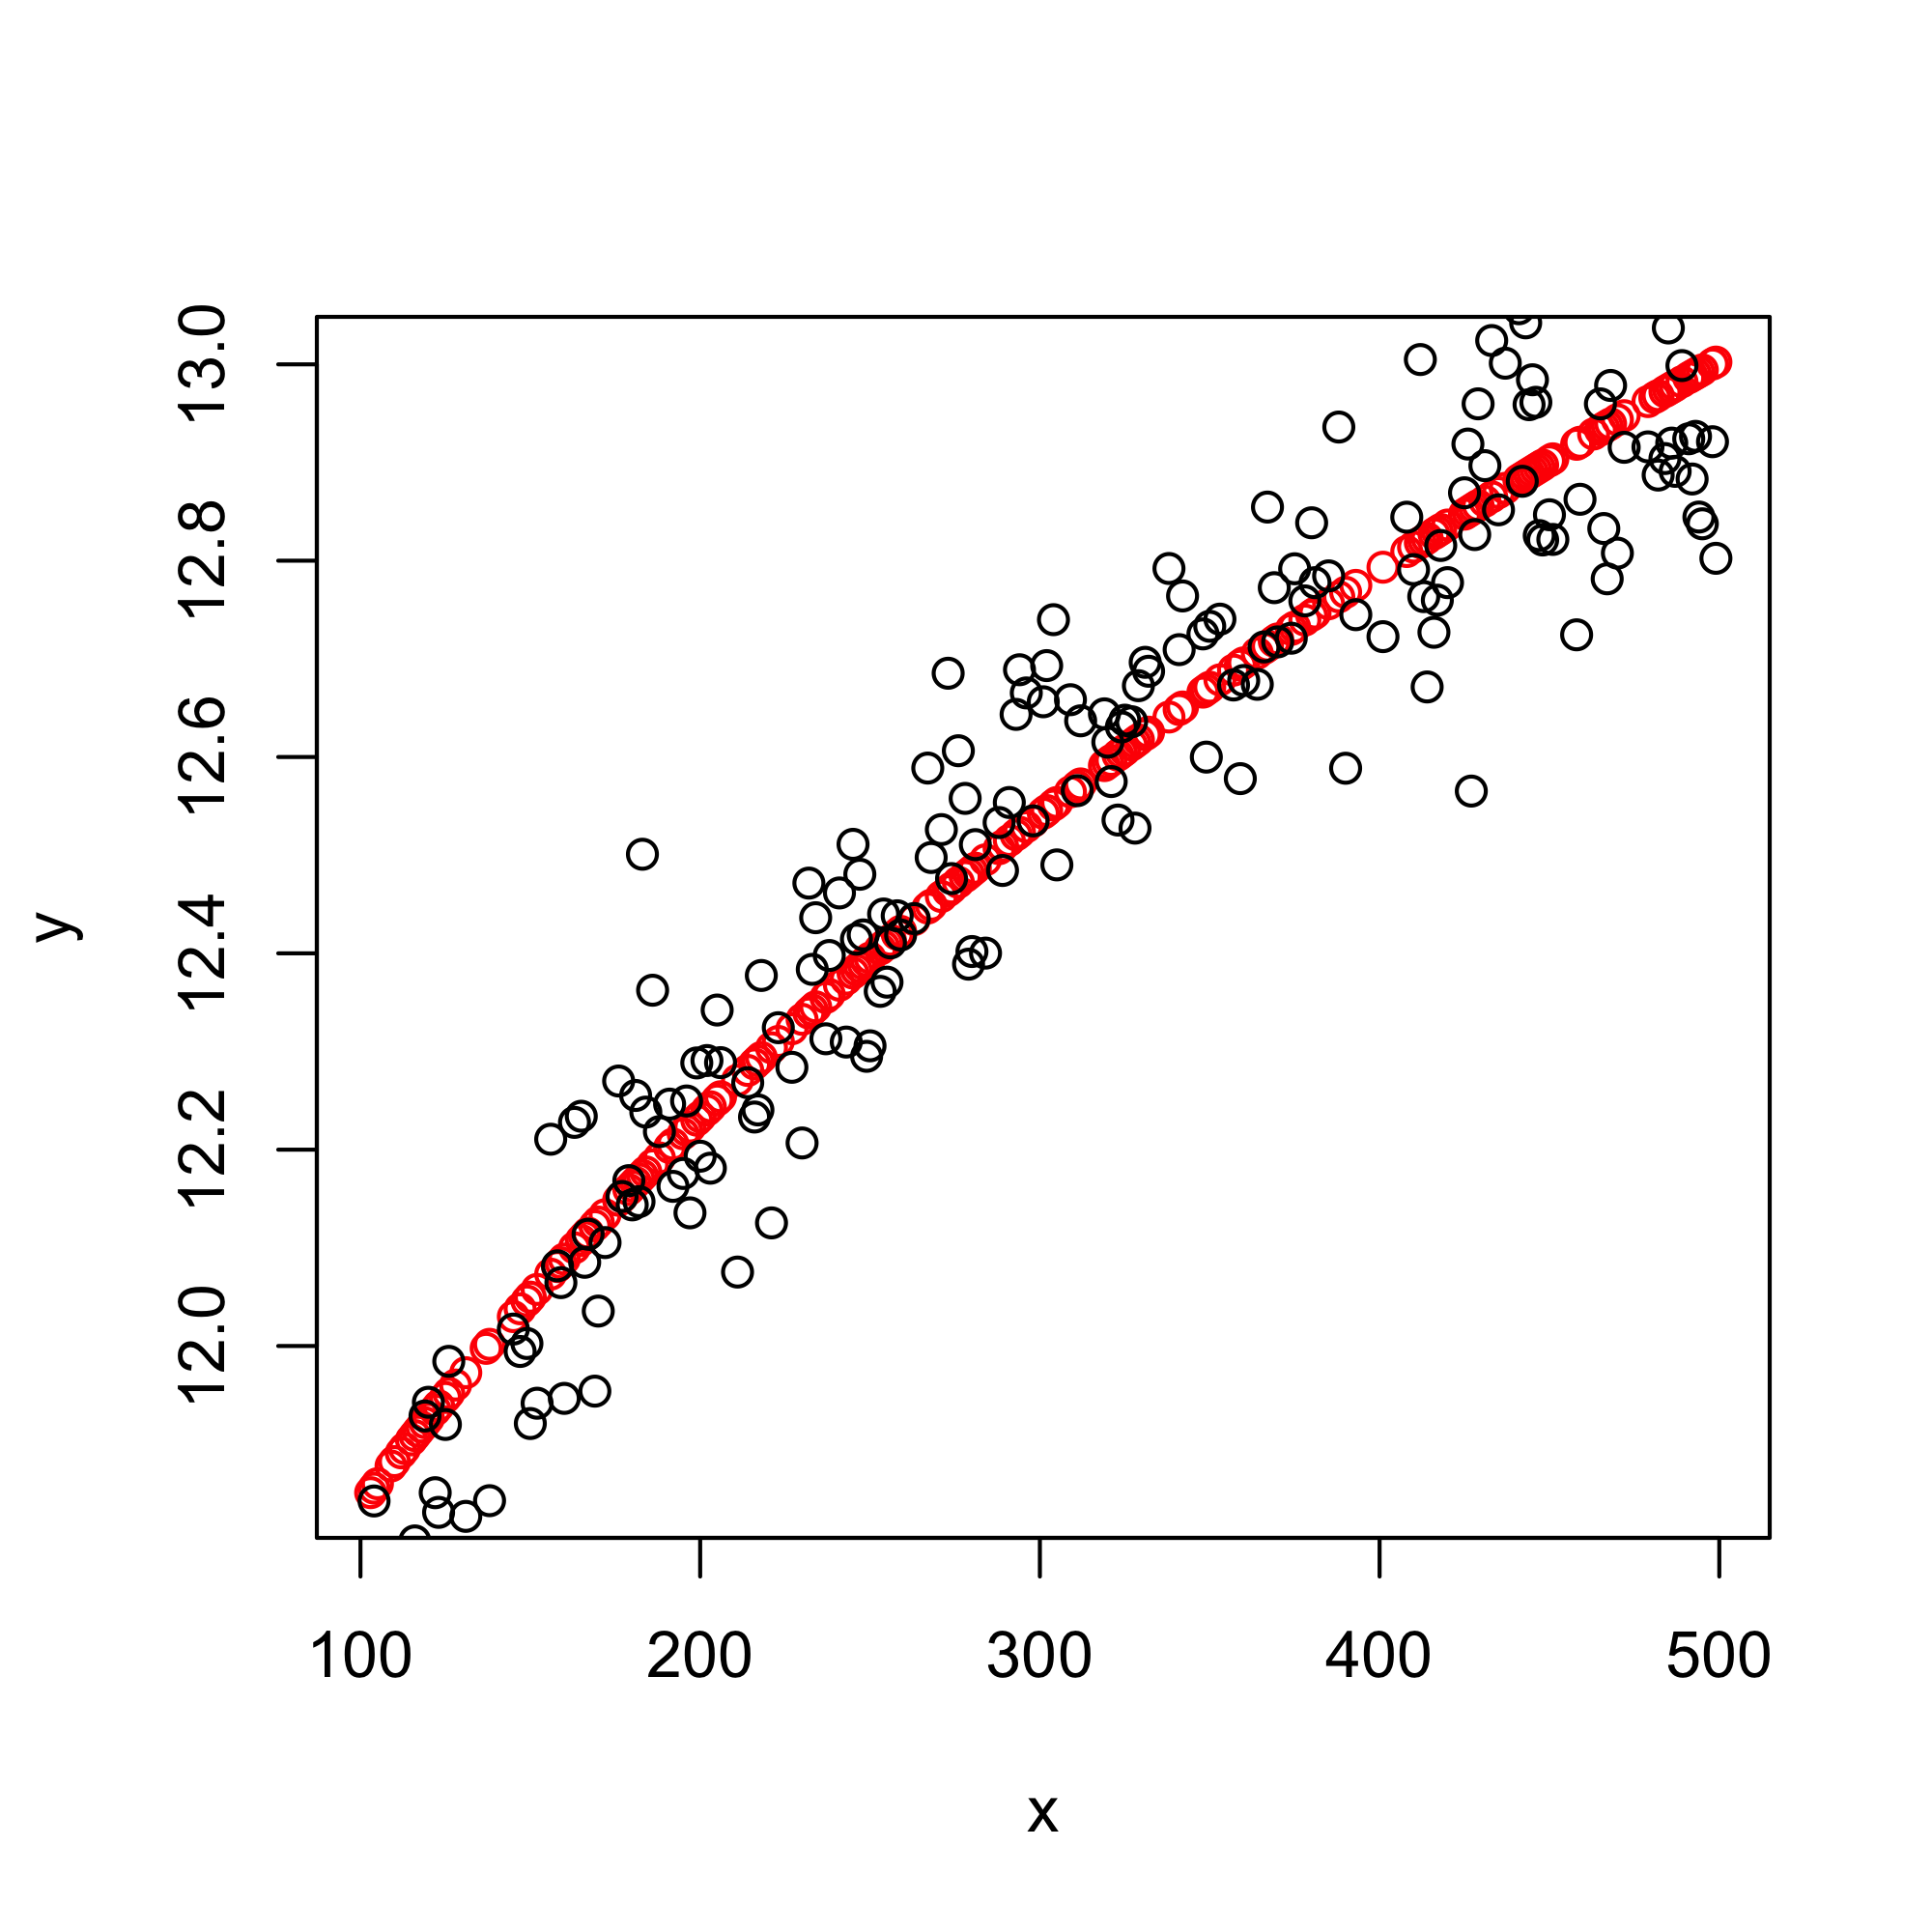
\includegraphics[width=\linewidth]{fit_x_log.png}
		\caption{In black, $y = .8 \log(x) + 8 + N$, and in red, a curve fitted with $\lambda = 10$.}
		\label{fig:fits_xy_log}
	\end{subfigure}
	\hfill
	\begin{subfigure}{0.45\linewidth}
		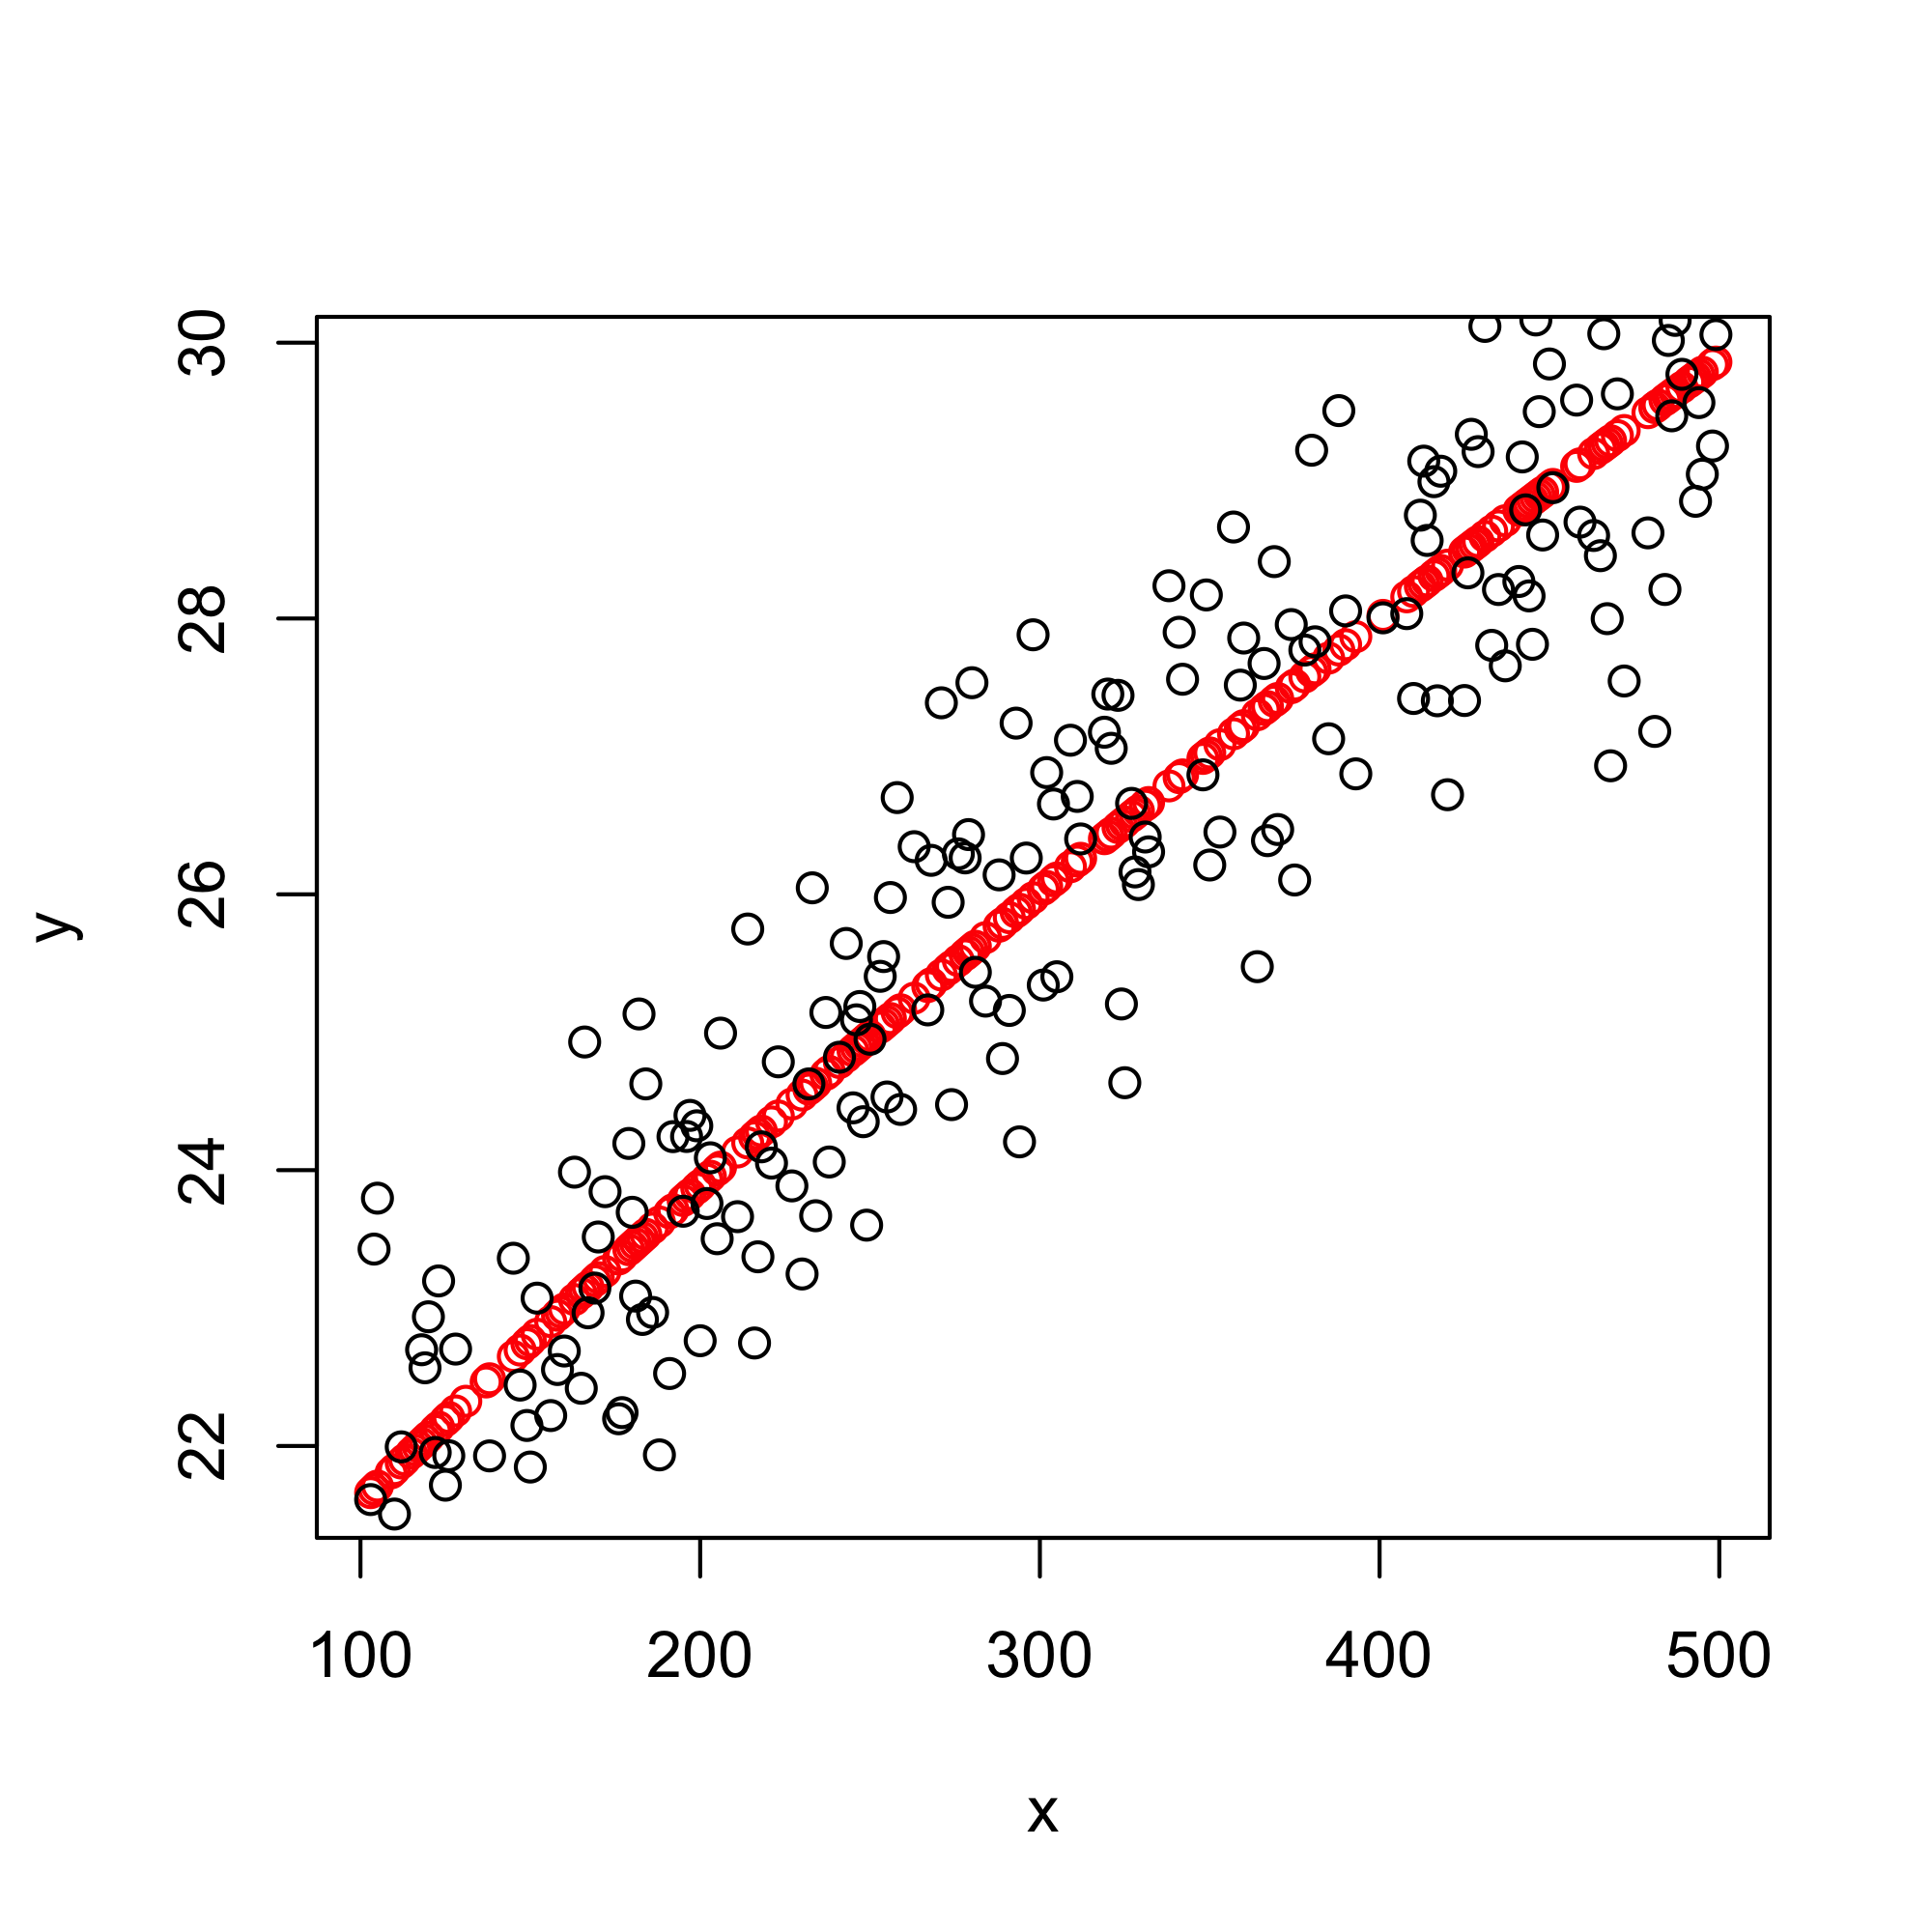
\includegraphics[width=\linewidth]{fit_x_sq.png}
		\caption{In black, $y = .7 \sqrt{x} + 14 +N $, and in red, a curve fitted with $\lambda = 1.85$.}
		\label{fig:fits_xy_sq}
	\end{subfigure}
	\caption{Data and curves fitted.} 
	\label{fig:fits_xy}
\end{figure}

The capabilities of R's \texttt{lm} function extends to multilinear regression. In order to exemplify this, three different sets of independent variables were created, and a variable dependent on these three was computed. The code where this is done, and its results, are shown in Listing \ref{lst:multilinear}.
 
\begin{lstlisting}[language=R, caption={Multilinear regression with \texttt{lm}.}, label={lst:multilinear} ]
x1 <- sample(x = 100:500, size = 200, replace = FALSE)

x2 <- sample(x = 200:600, size = 200, replace = FALSE)

x3 <- sample(x = 100:500, size = 200, replace = FALSE)

my2 <- 3*x1 + .5*log(x2) + 5*x3

lm(my2 ~ x1 + log(x2) + x3)

#Call:
#lm(formula = my2 ~ x1 + log(x2) + x3)

#Coefficients:
#(Intercept)           x1      log(x2)           x3  
#2.187e-12    3.000e+00    5.000e-01    5.000e+00  
\end{lstlisting}

\subsection{Vehicles in circulation in Mexico}
In this subsection, a curve is fitted to real data. The number of vehicles in circulation in Mexico per year, from 1986 to 2019, is downloaded from INEGI's webiste \cite{inegi}. A fragment of the data can be seen in Table \ref{tab:vehicles}. The data is also shown in Figure \ref{fig:vehicles}.
Two distinct approaches are taken here. The first approach consists of using the function \texttt{choose\_lambda}, which gives a value $\lambda$ to transform the data as was done in Section \ref{analysis}. A value of $\lambda = -0.201$ is obtained. As before, a linear model is fitted for $(x, \tilde{y}_\lambda)$. The function obtained with this method is $y = (0.8393 - 0.0004 x)^{-1/0.201}$, and it can be seen in Figure \ref{fig:fit_vehicles}.  The second approach consists of assuming the number of vehicles in circulation has exponential growth, and fitting a curve with \texttt{lm(log (y) $\sim$ x)}. This gives a model $y = \exp(0.0568 - 97.1138x)$, and can be seen in Figure \ref{fig:fit2_vehicles}. This second model is also used to plot a $99\%$ confidence interval for the data, as seen in Figure \ref{fig:predicted_intervals_vehicles}.
% latex table generated in R 4.0.0 by xtable 1.8-4 package
% Sun Oct 18 19:27:24 2020
\begin{table}
	\centering
	\caption{Vehicles in circulation in Mexico.}
	\begin{tabular}{rrr}
		\hline
		& year & vehicles \\ 
		\hline
		1 & 1981 & 6,339,836 \\ 
		2 & 1982 & 6,695,164 \\ 
		3 & 1983 & 6,941,252 \\ 
		4 & 1984 & 7,305,066 \\ 
		5 & 1985 & 7,725,623 \\ 
		6 & 1986 & 7,732,012 \\ 
		\hline
	\end{tabular}
	\label{tab:vehicles}
\end{table}



\begin{figure}
	\centering
	\begin{subfigure}{.45 \linewidth}
		\centering
		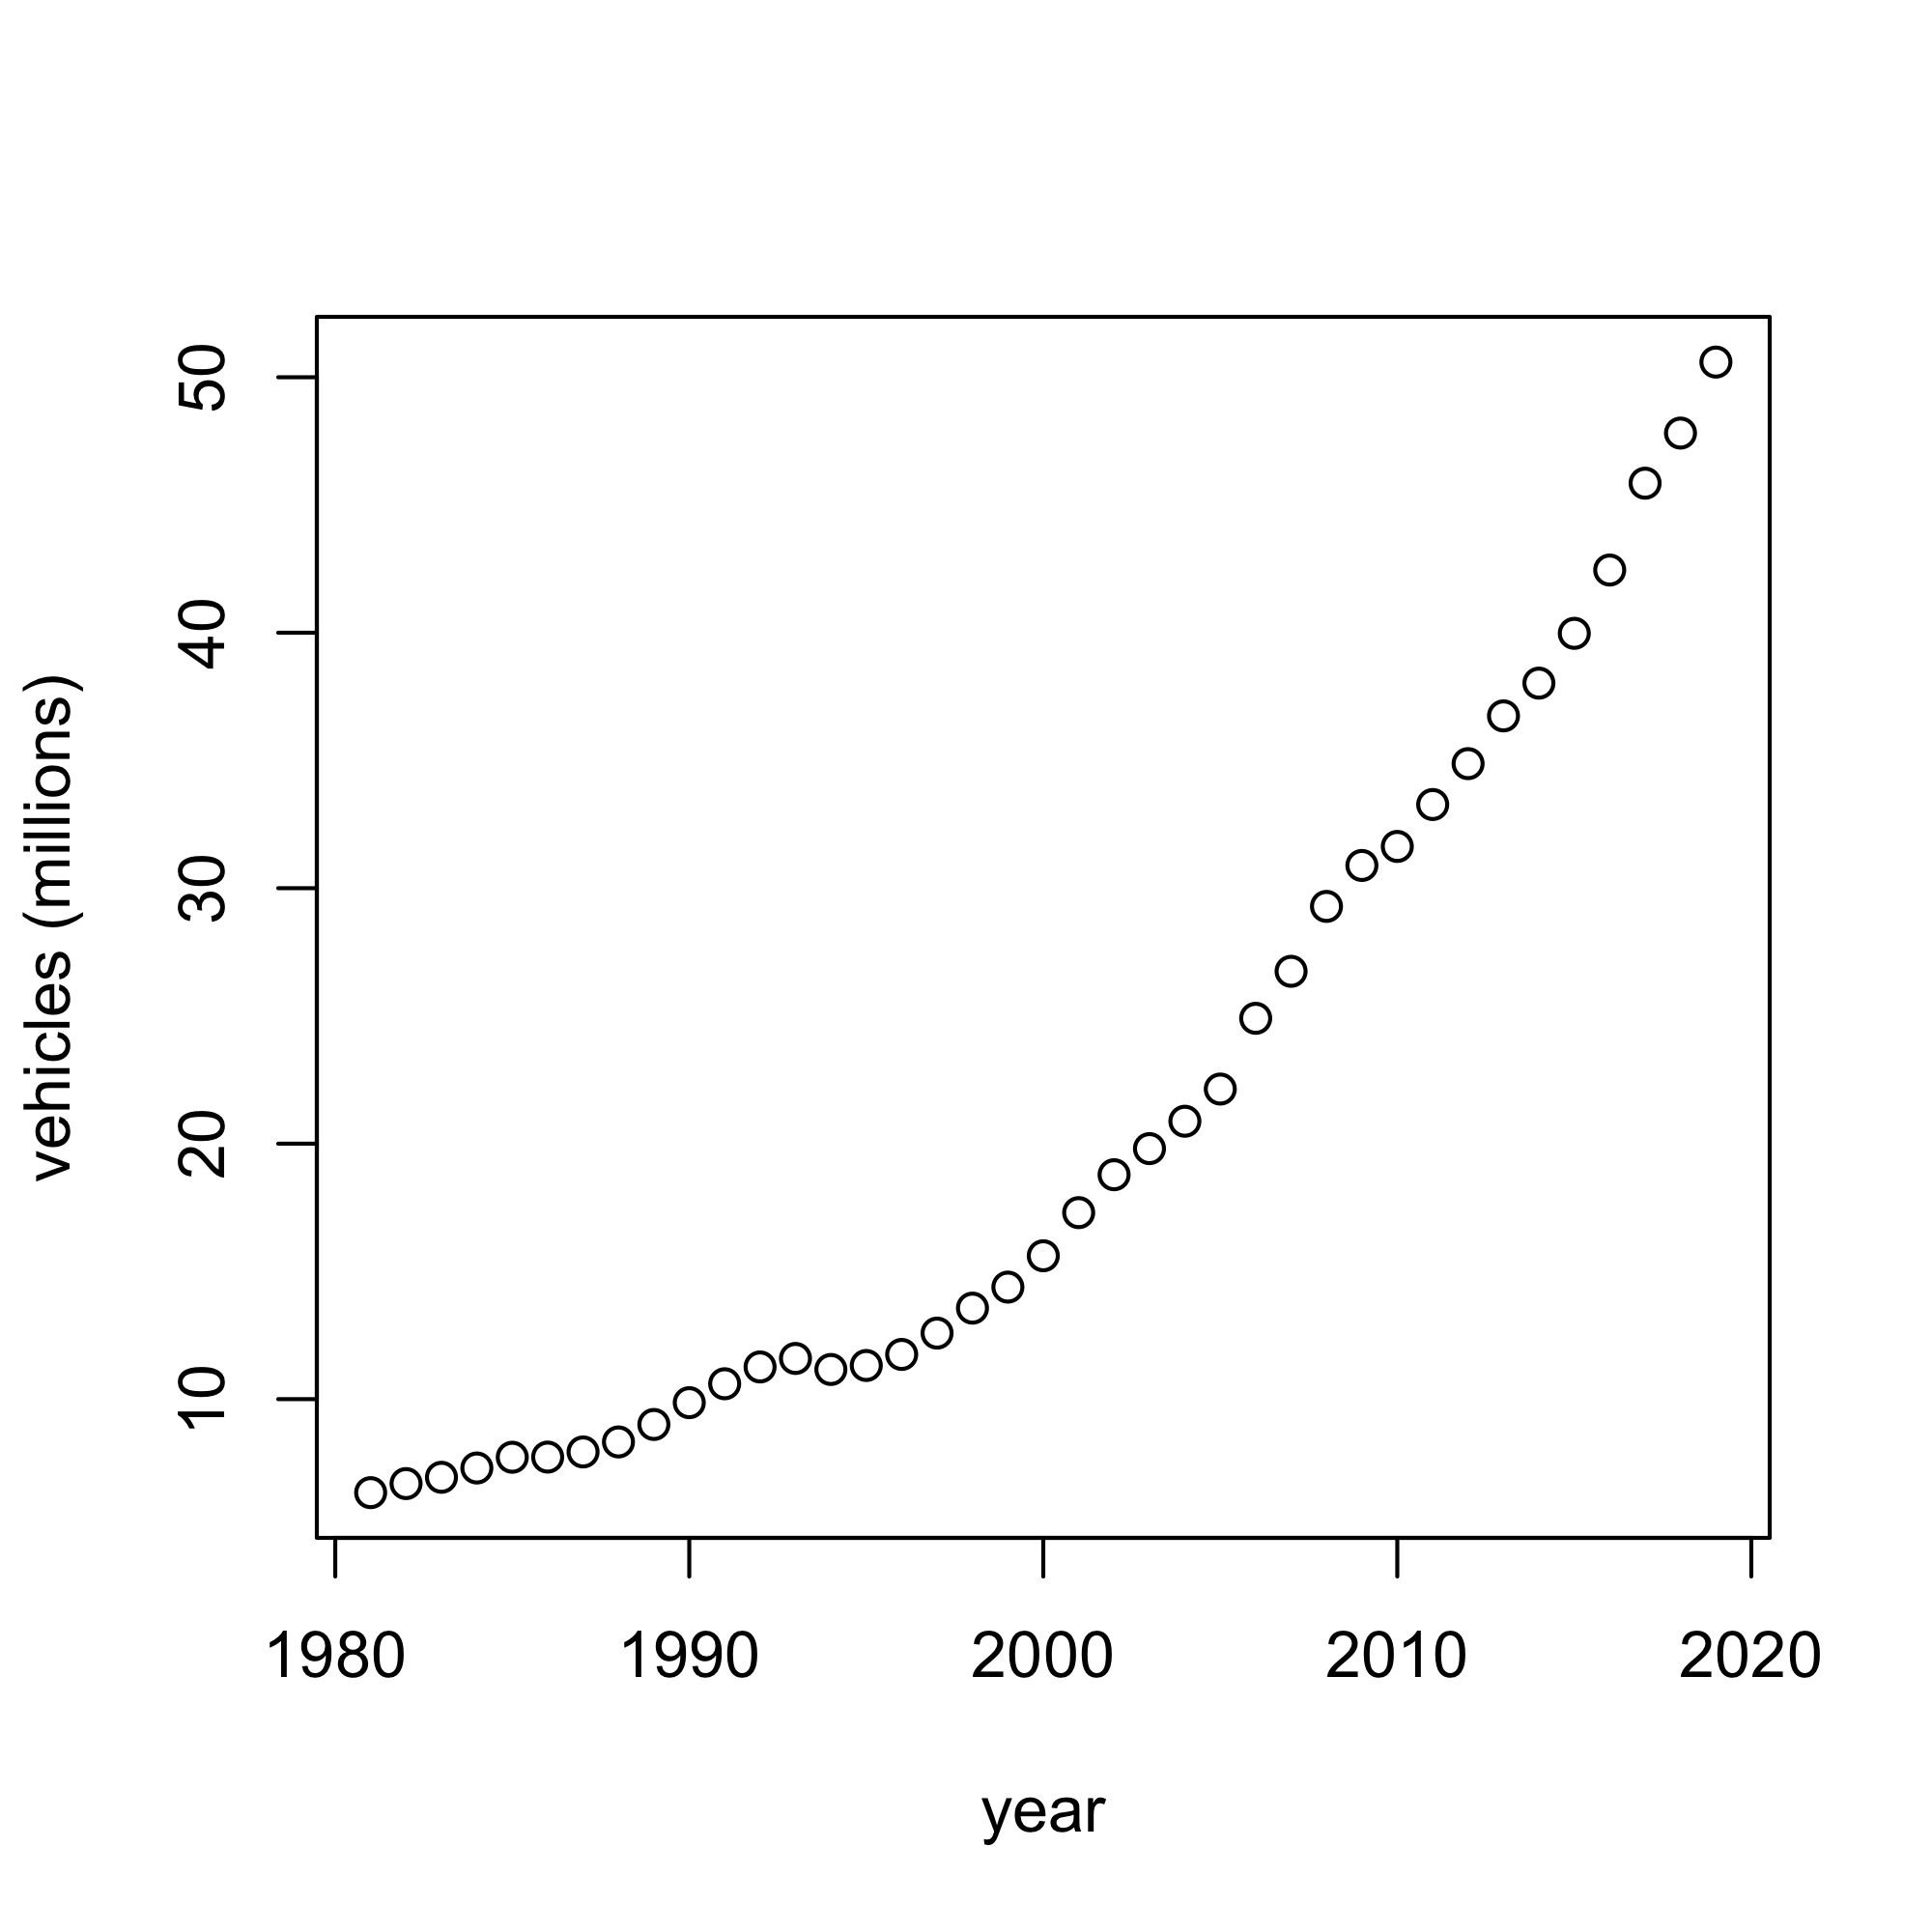
\includegraphics[width=\linewidth]{vehicles_year.png}
		\caption{Vehicles in circulation per year.}
		\label{fig:vehicles}
	\end{subfigure}
	\hfill
	\begin{subfigure}{0.45\linewidth}
		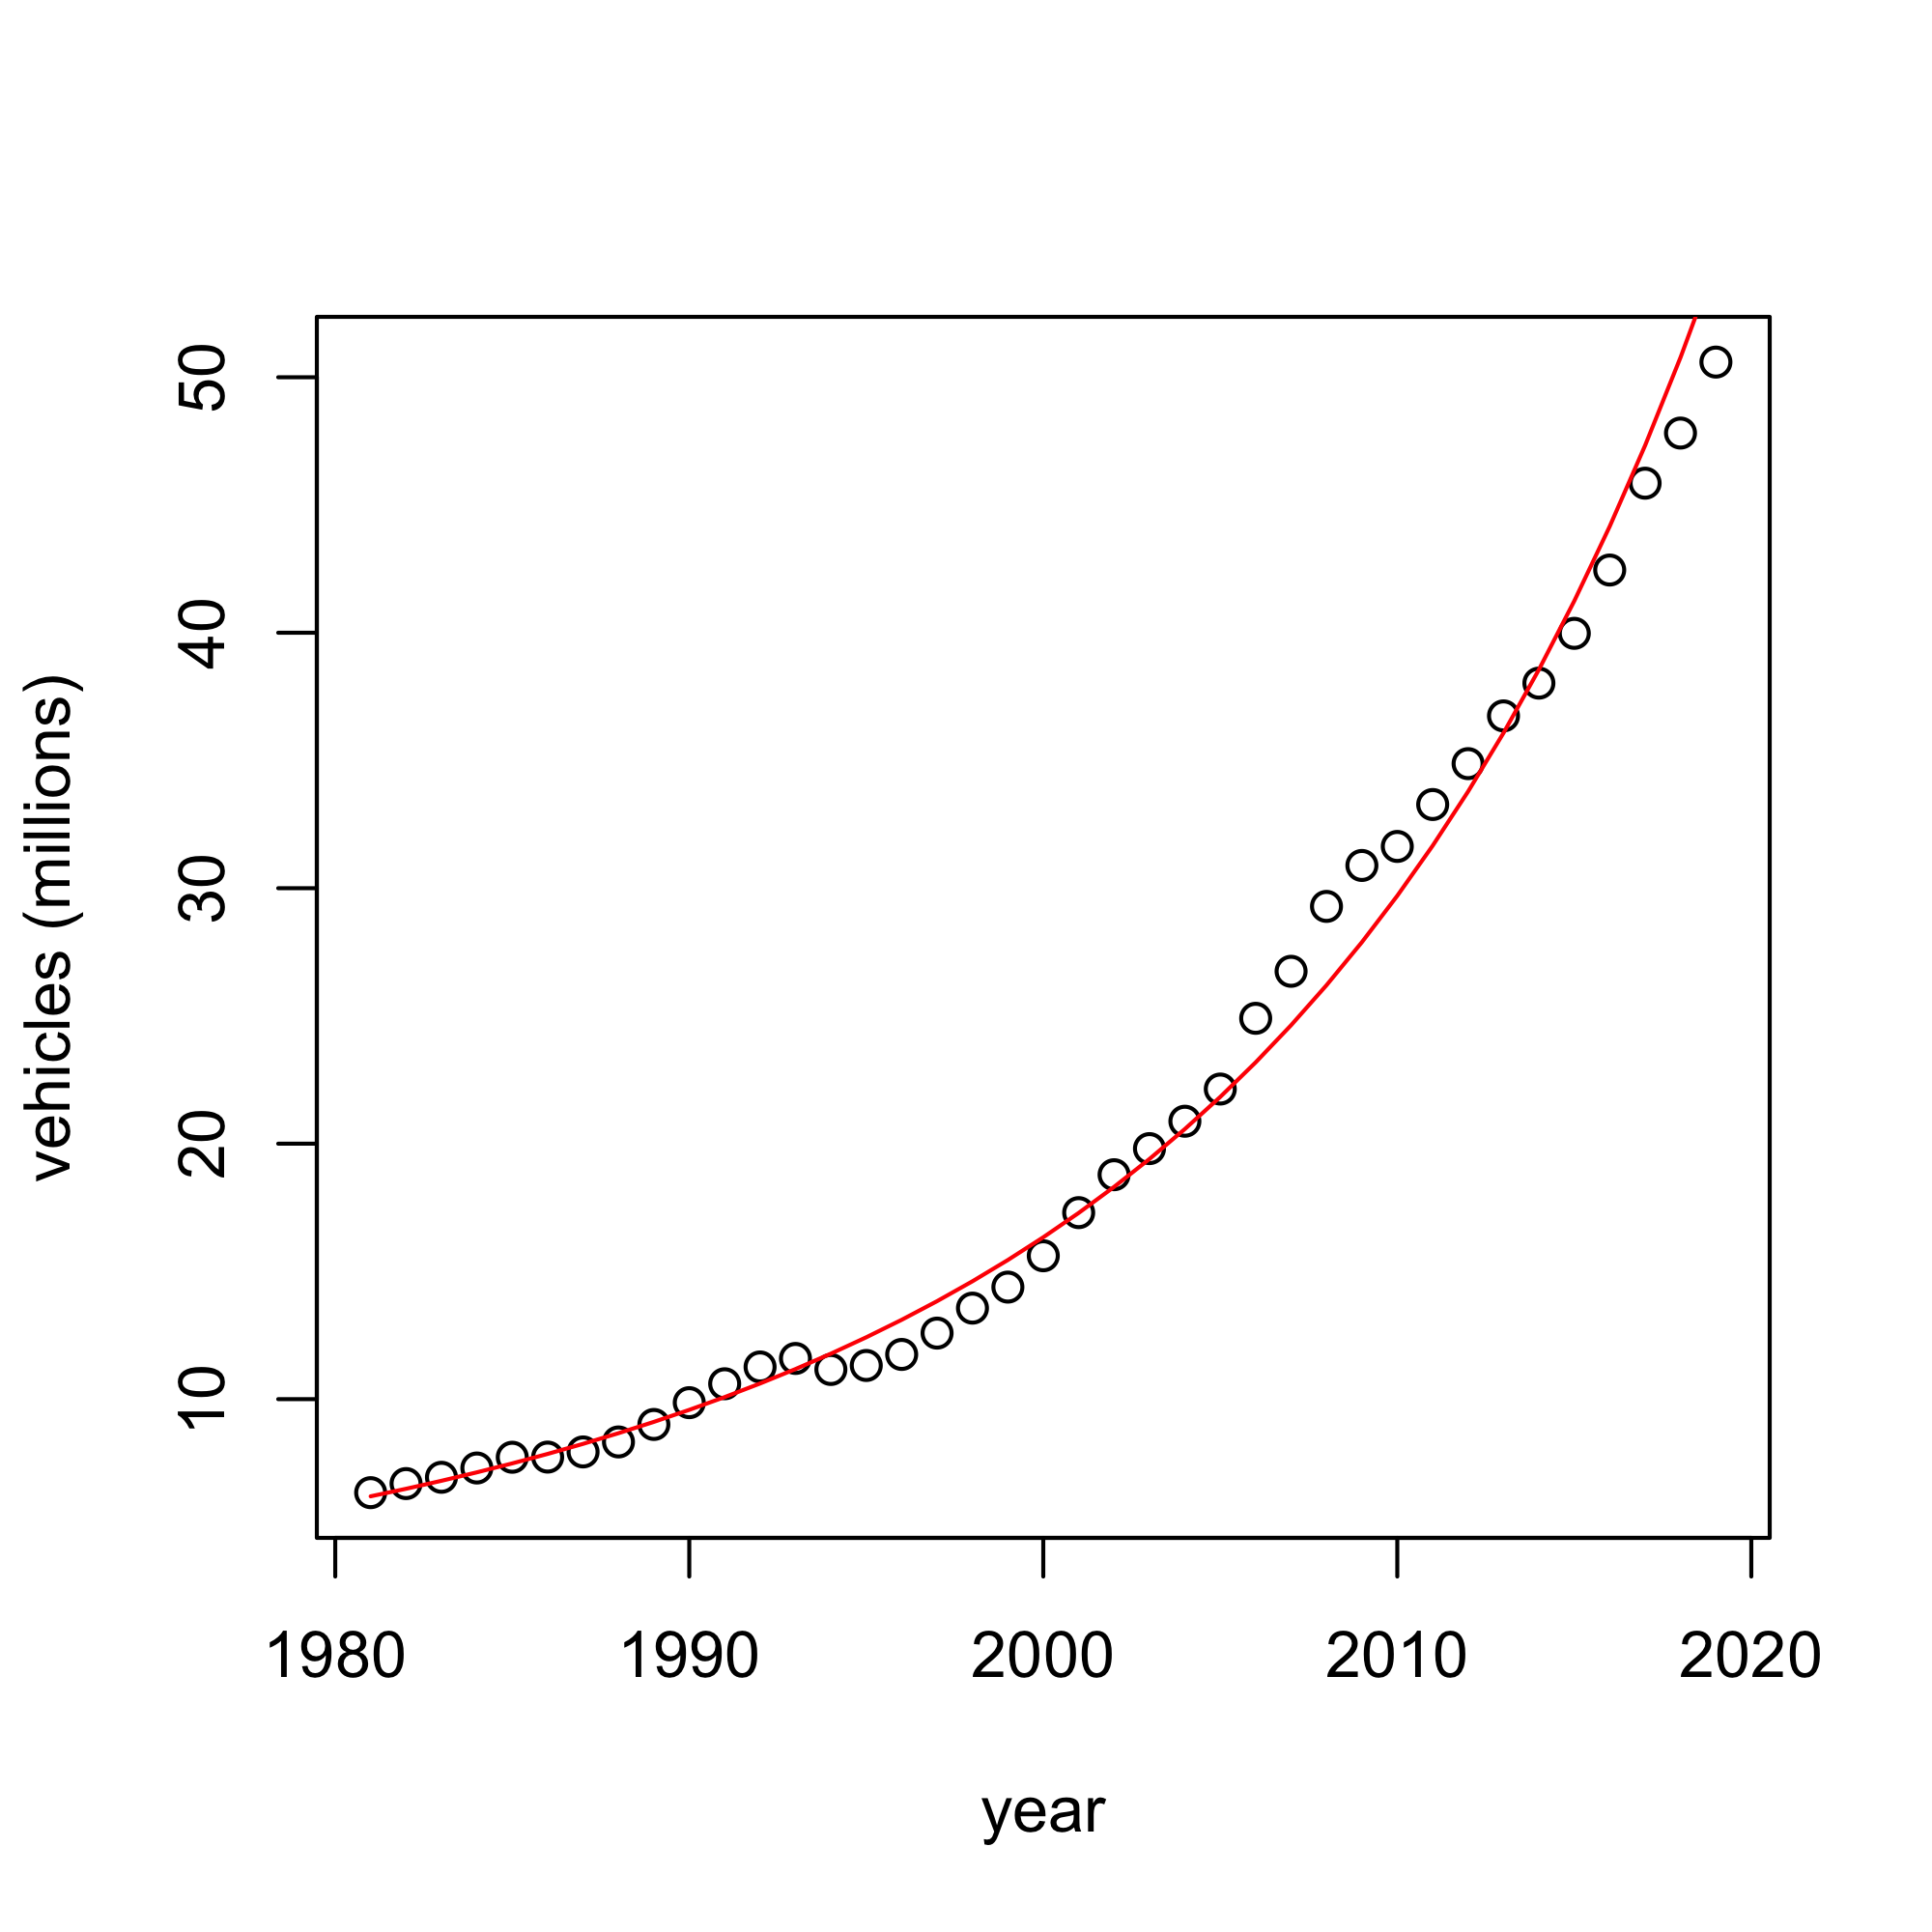
\includegraphics[width=\linewidth]{fit_vehicles_year.png}
		\caption{Vehicle data (black) and $y = (0.8393 - 0.0004 x)^{-1/0.201}$ (red).}
		\label{fig:fit_vehicles}
	\end{subfigure}
	\hfill
	\begin{subfigure}{0.45\linewidth}
		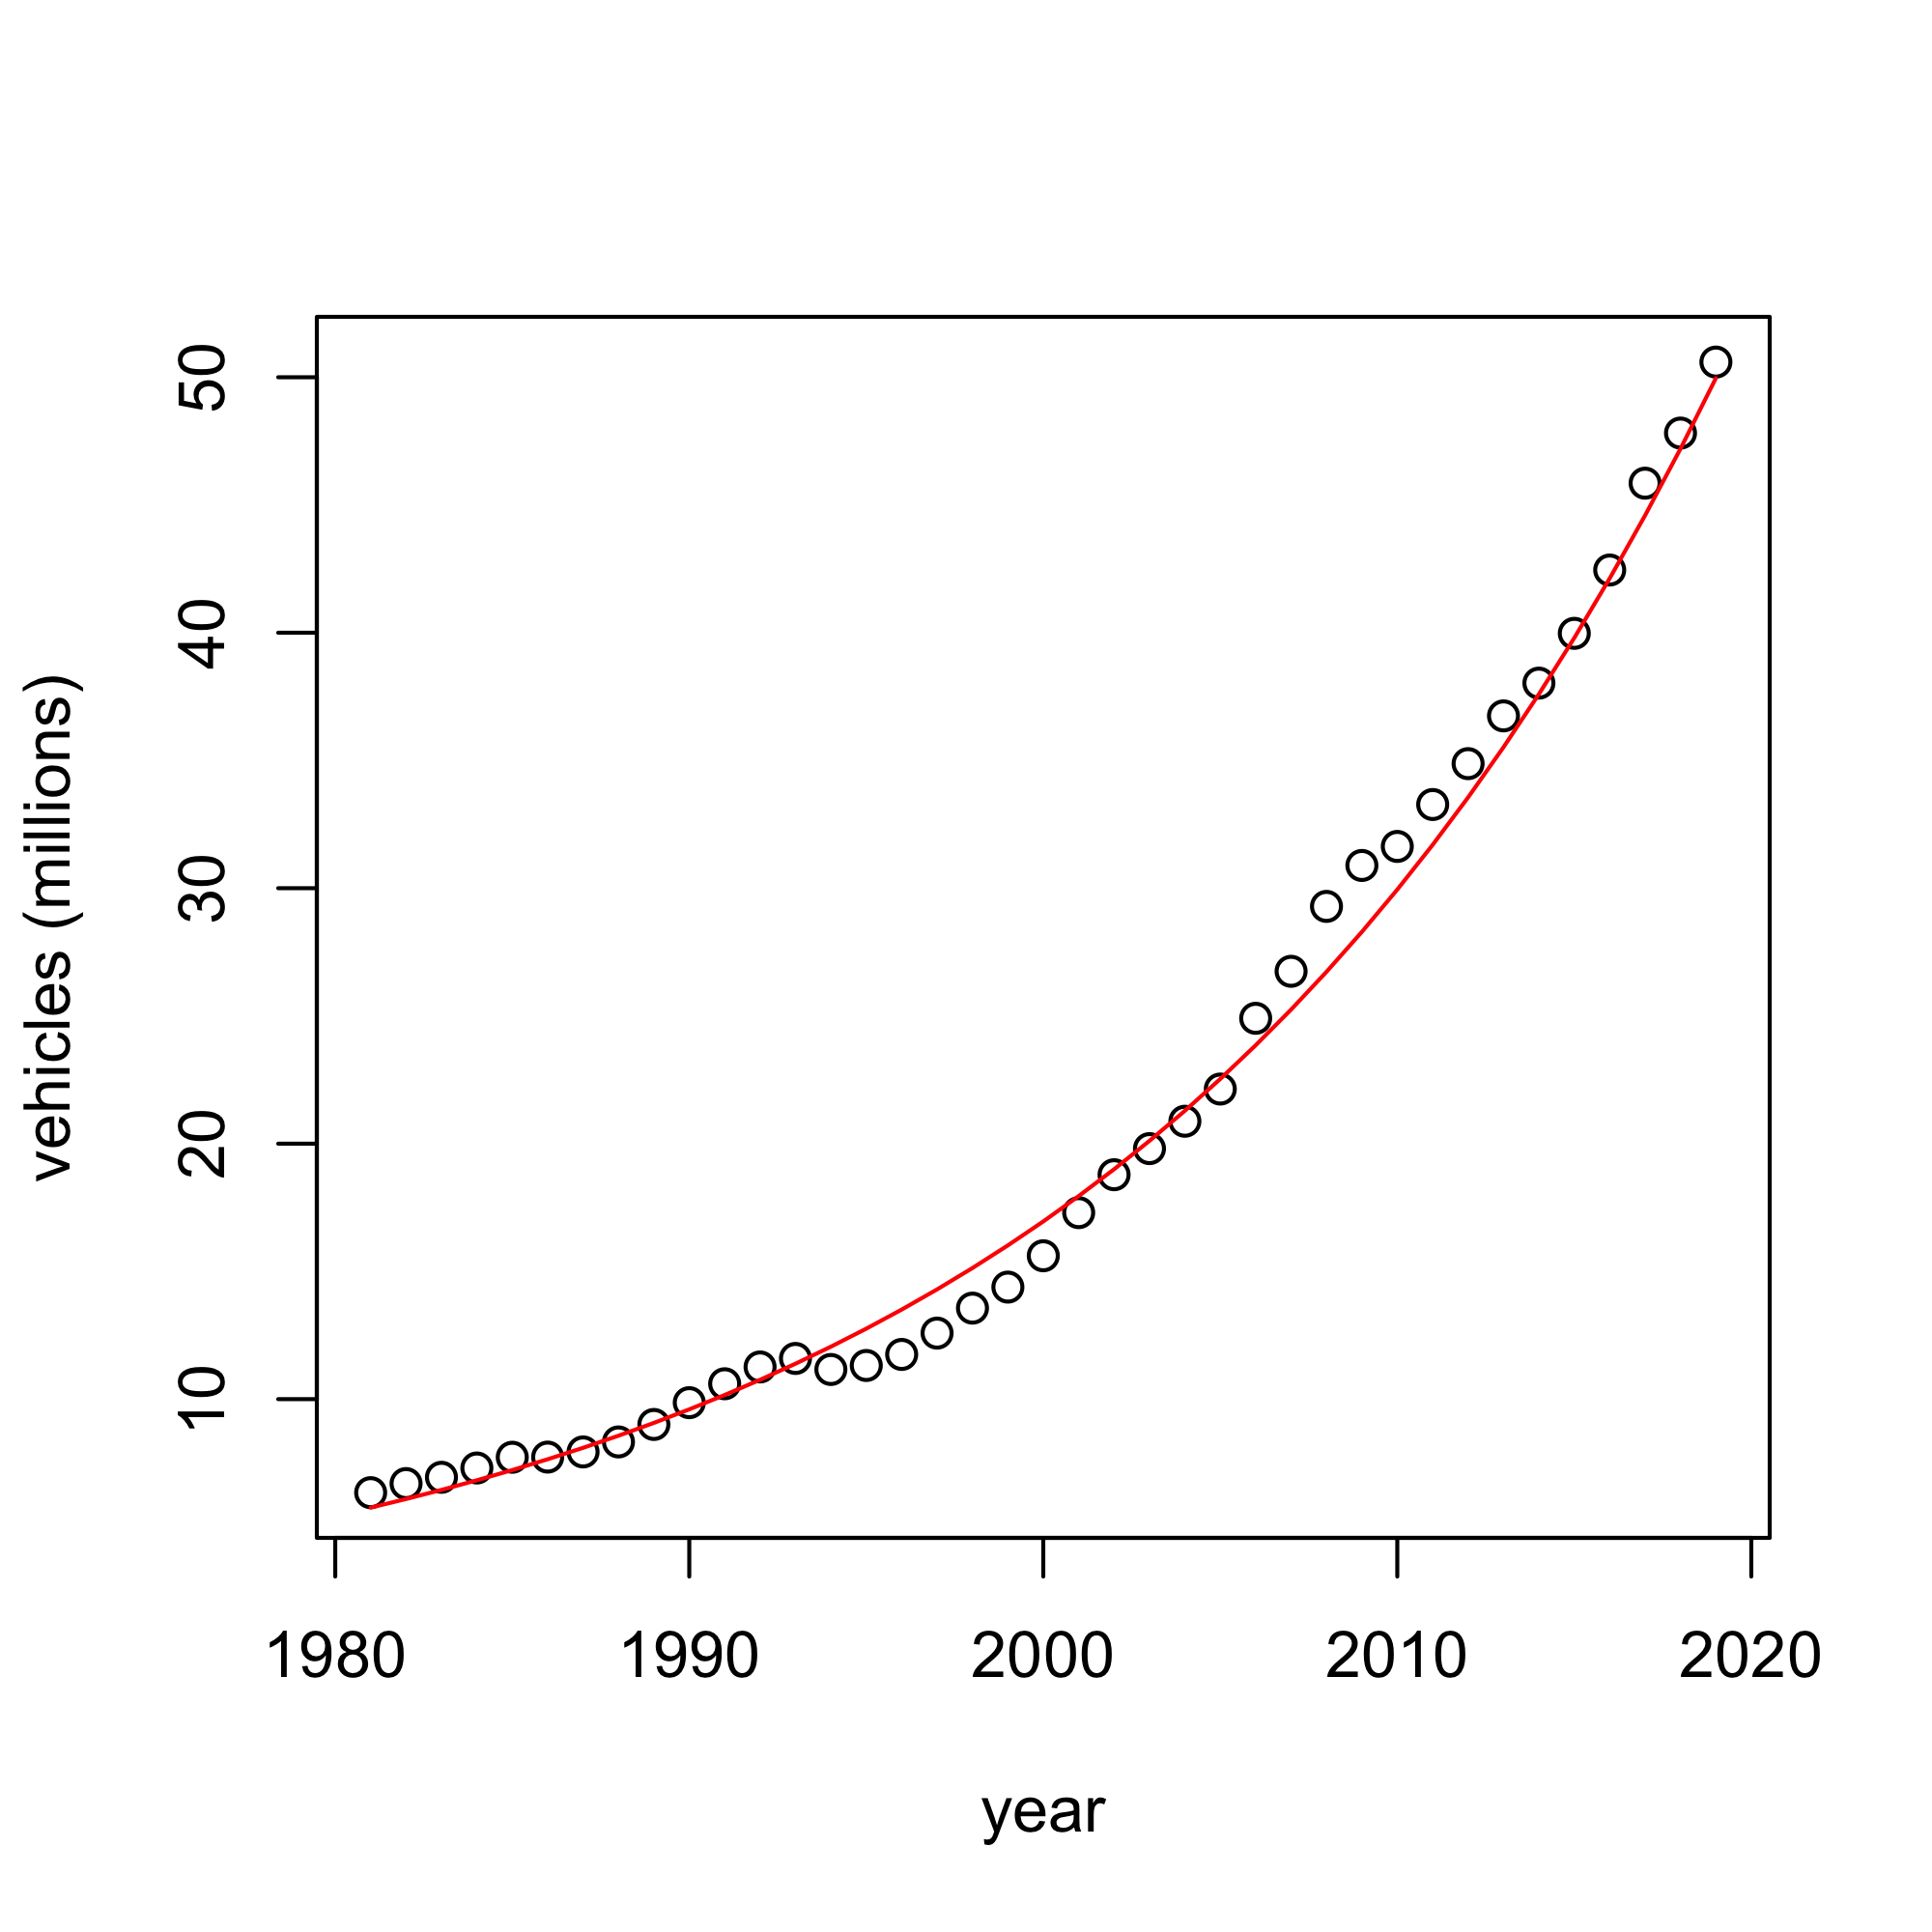
\includegraphics[width=\linewidth]{fit2_vehicles_year.png}
		\caption{Vehicle data (black) and $y = \exp(0.0568 - 97.1138x)$ (red).}
		\label{fig:fit2_vehicles}
	\end{subfigure}
	\hfill
	\begin{subfigure}{0.45\linewidth}
		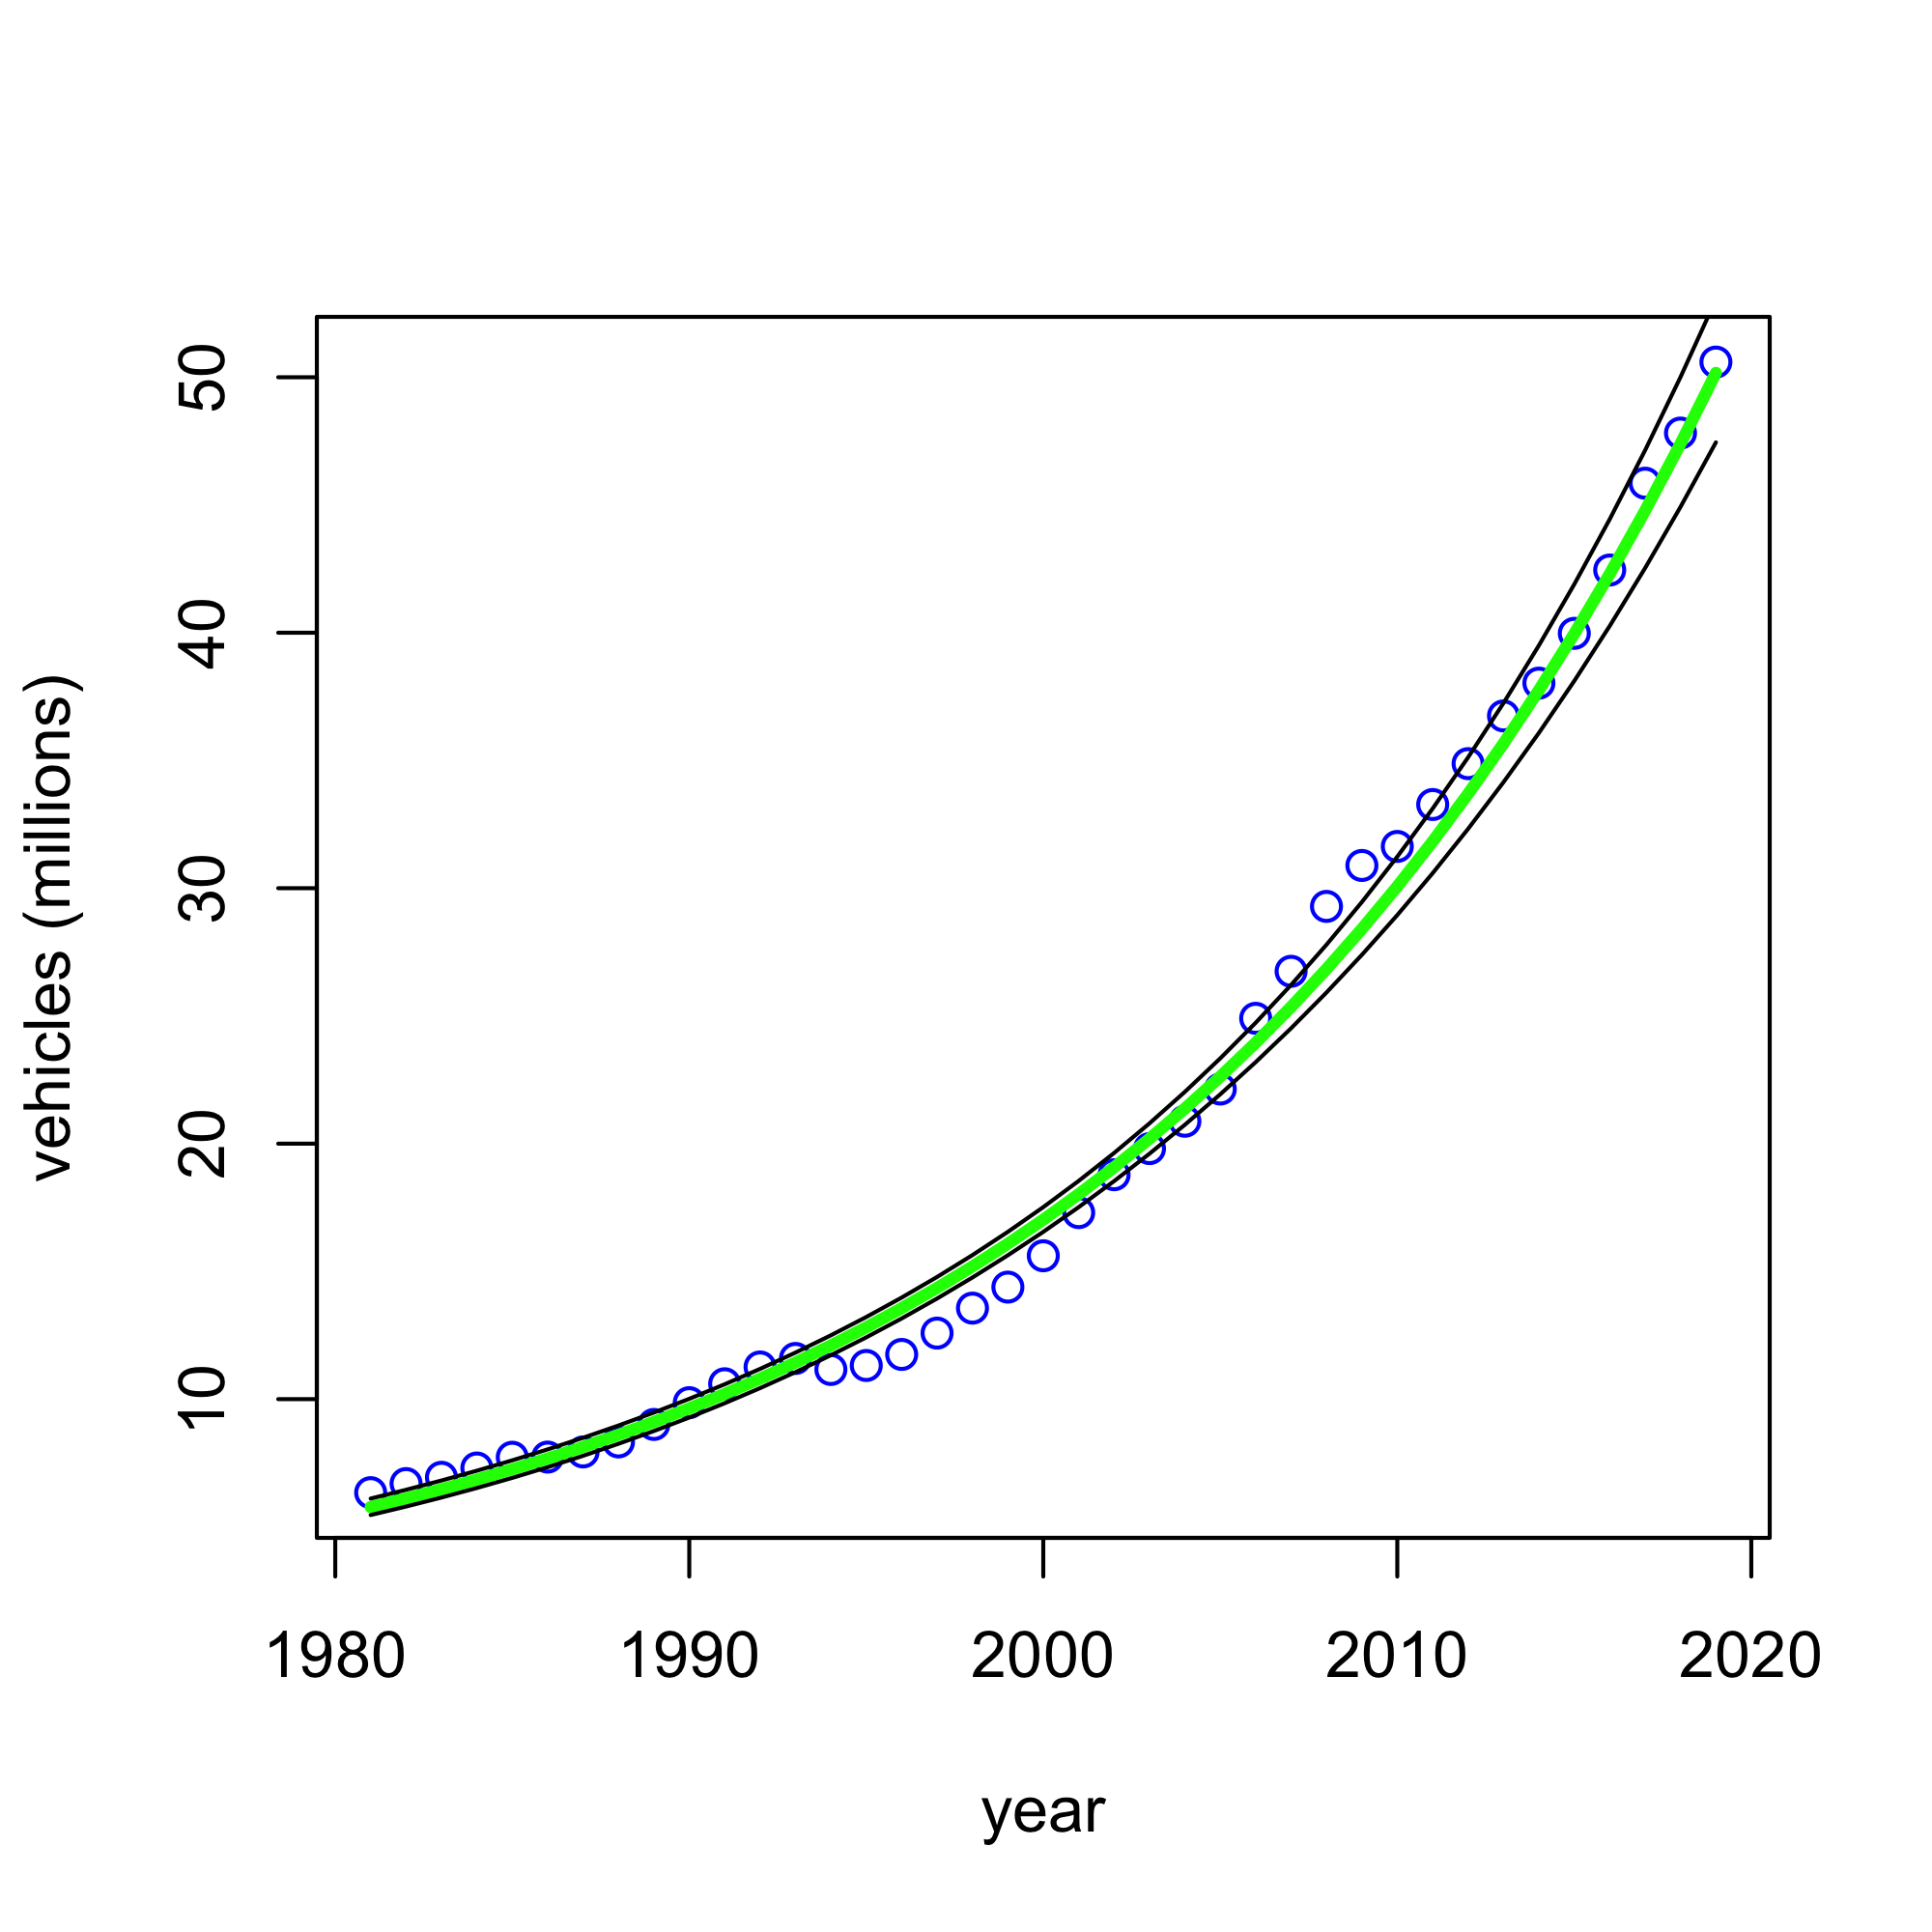
\includegraphics[width=\linewidth]{predicted_intervals_vehicles_year.png}
		\caption{Vehicle data (blue) and predicted intervals (black and green).}
		\label{fig:predicted_intervals_vehicles}
	\end{subfigure}
	\caption{Models for vehicle data.} 
	\label{fig:models_vehicles}
\end{figure}

\section{Conclusion}
The theory and methods of curve fitting is larger than what was presented here. Many other techniques can be applied and studied further, for example, fitting a model on real data with more than one independent variable. Models including non-uniform independent variables can also be studied.

%%%%%%%%%%%%%%%%%%%%%%%%%%%%

\bibliographystyle{siam}
\bibliography{refr}


%%%%%%%%%%%%%%%%%%%%%%%%%%%%
\end{document}
